\chapter{Prototype Systems}
\label{prototypes}

Over the past several years we have been exploring various means of creating a
child-friendly tangible user interface that would serve as an input device for
exploring 3D modeling and digital fabrication. To this end, we have created
three prototypes: the UCube, an initial proof-of-concept device, SnapCAD, a more
expressive and study iteration of the UCube, and PopCAD a paper-based interface
addressing several of the concerns raised by SnapCAD. These systems all
communicate with versions of a companion software program running on  desktop
computer. This chapter describes these systems, the motivations behind their
design, and the technical work involved in their creation.

\section{UCube}

The UCube represents our first attempt to create a cooperative system of
hardware and software that encapsulated and combined our beliefs about embodied
cognition and the importance of accessible digital fabrication. The idea for the
UCube originally came from the attempt to create a ``3D Geoboard''.
\autoref{fig:geoboard} shows a rudimentary 2D geoboard consisting of a 3x3 grid
of nails stuck into a wooden block. Simple geometries, such as the triangle shown
in the referenced image, can be made by stretching rubber bands around some
number of ``pegs''. The geoboard invites a kind of tangible, exploratory, and
embodied play that (as we discuss in Chapter 3) promotes children's learning in
powerful ways. The goal, then, was to capture the ``gestalt'' of the traditional
2-dimensional geoboard and extend it - into 3-dimensions, and with a
computationally-enhanced interface that could translate physical modeling on a
device into a software program that could display the input from the geoboard in
a meaningful way.

\begin{figure}[ht]
\begin{center}$
\begin{array}{cc}
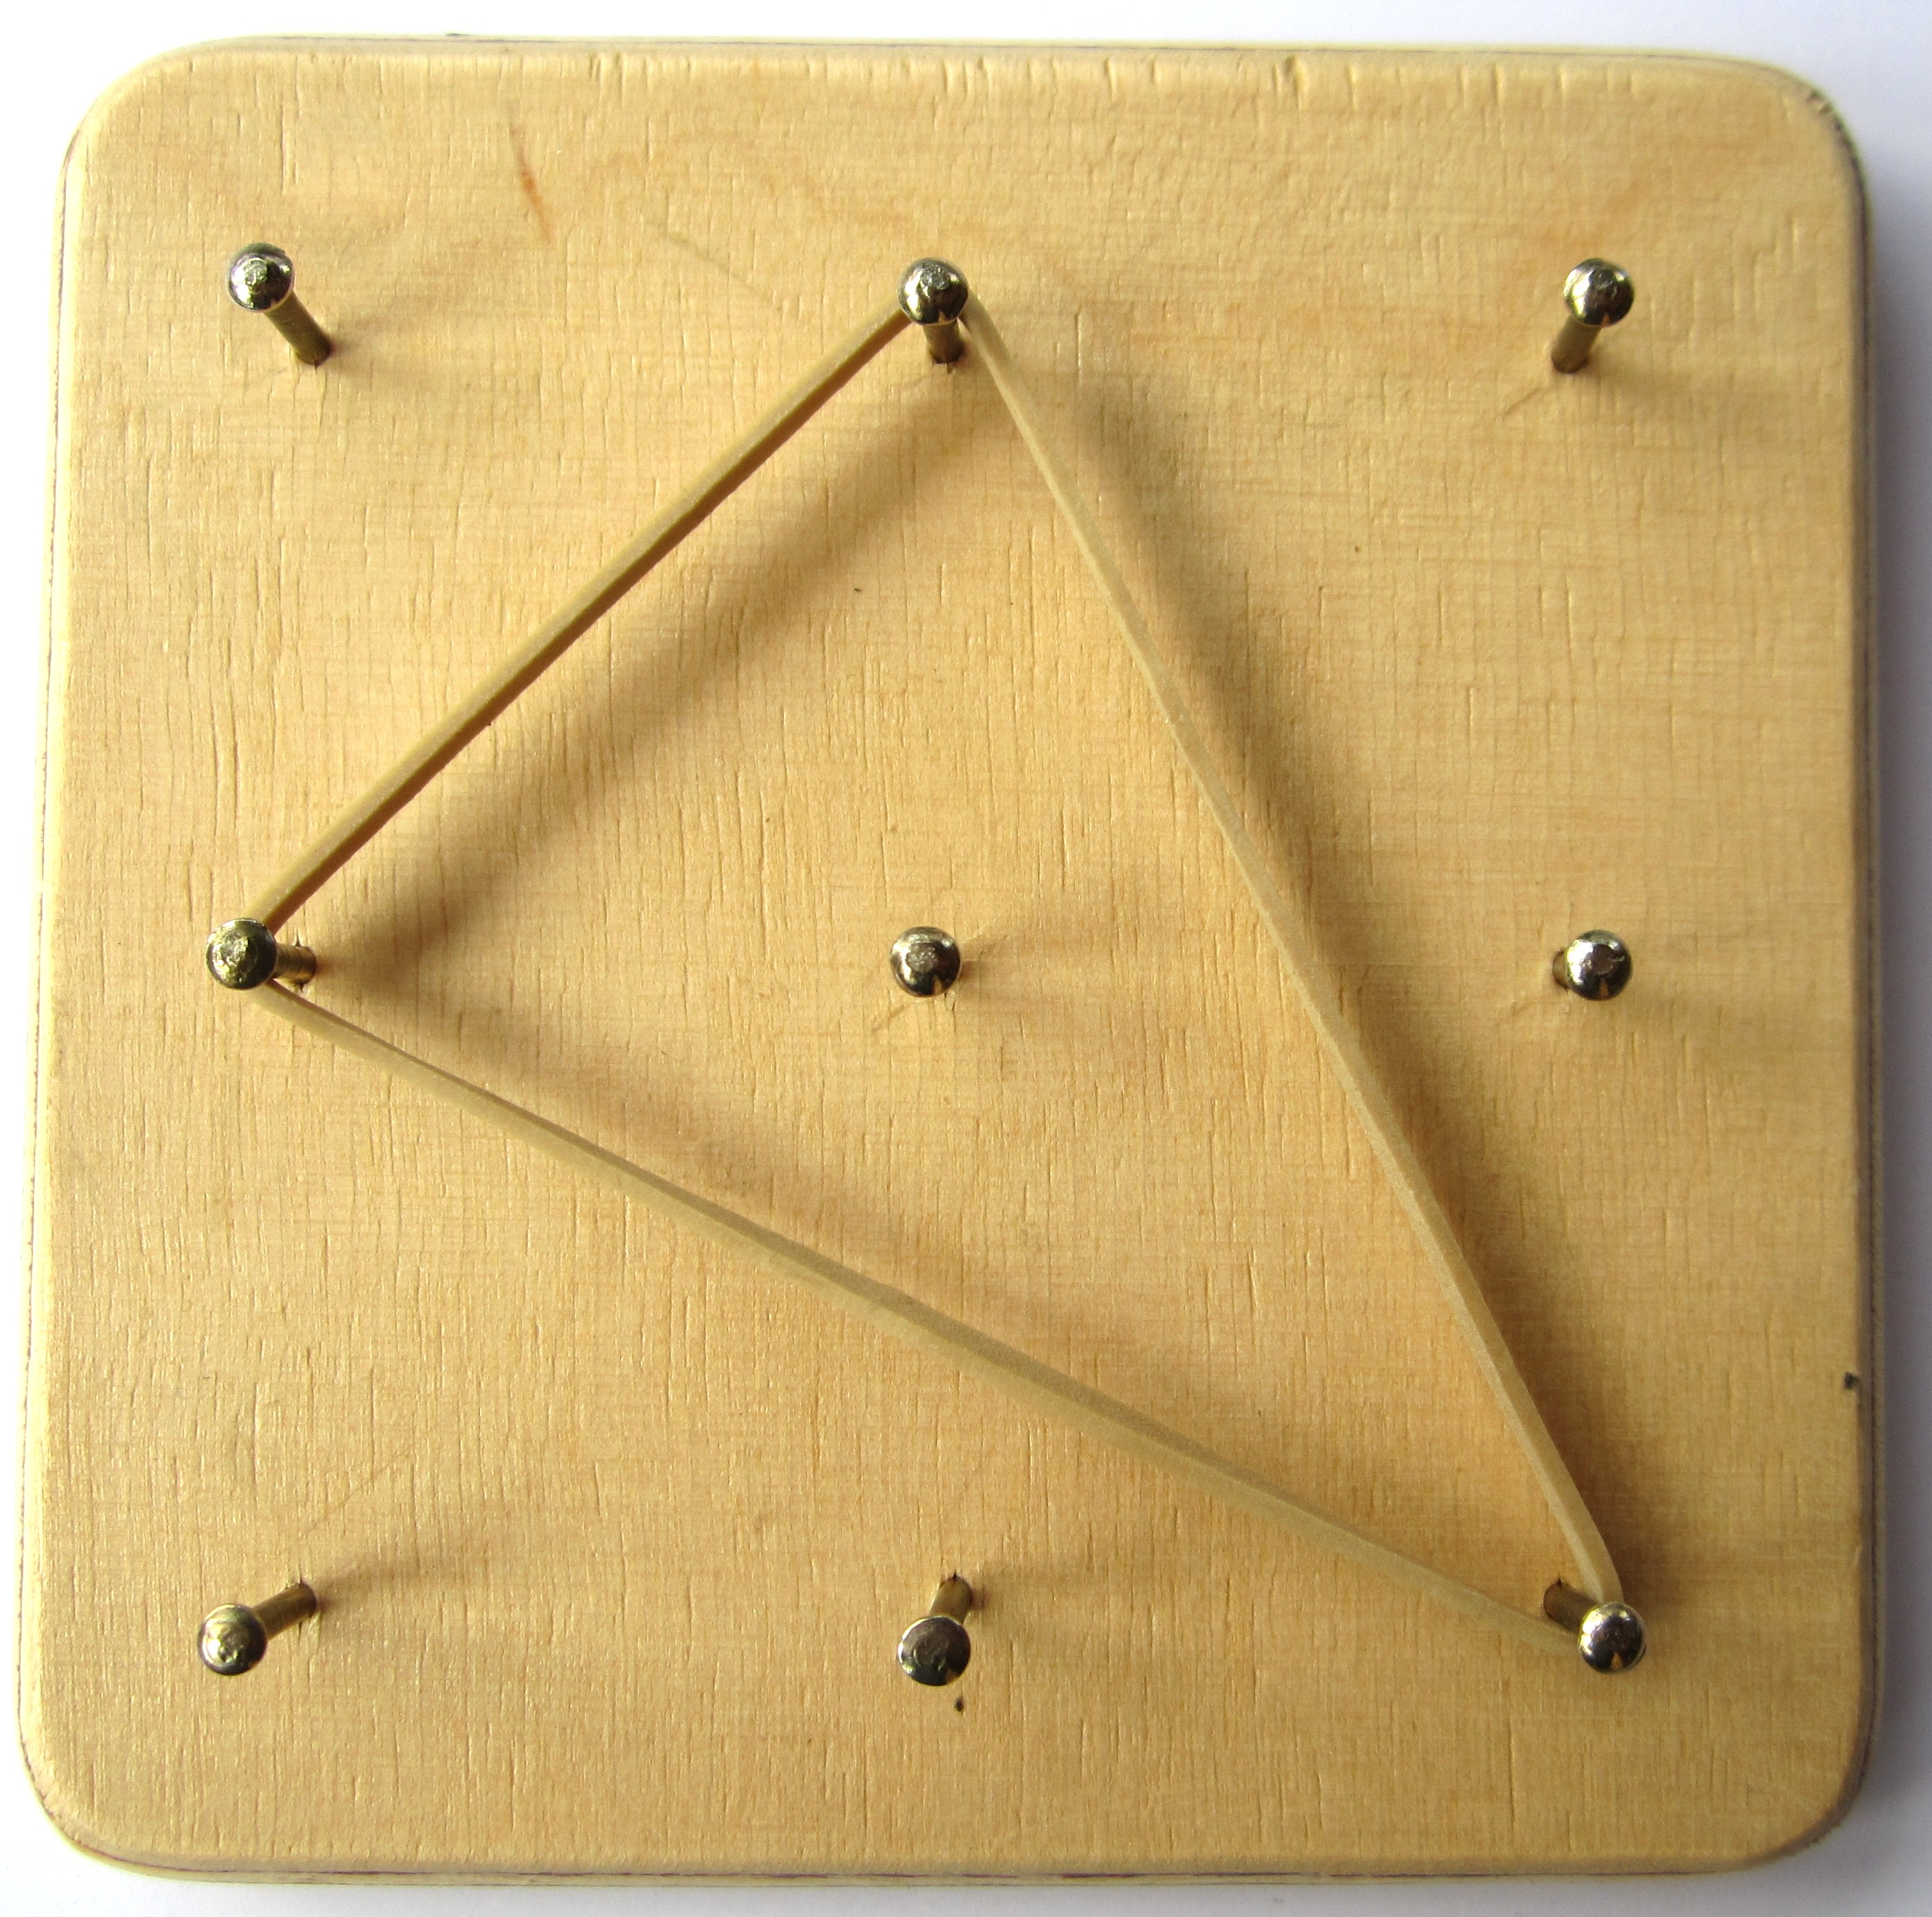
\includegraphics[width=.5\linewidth]{images/Geoboard}
\end{array}$
\end{center}
\caption{A simple 3x3 geoboard, with a rubber band stretched around several
pegs, forming a triangle.}
\label{fig:geoboard}
\end{figure}

The UCube (as seen on the left in \autoref{fig:cubev1}) was the initial result
of this goal. The physical interface consists of a set of vertical ``towers''
that are placed (and optionally re-placed) onto a board, acting somewhat like
the nails in the 2D geoboard. These towers are moved around a grid of 4x4 evenly
spaced nodes or sockets into which the towers are placed. The towers themselves
contain four switches placed vertically along the tower, creating a potential
for 64 (4x4x4) distinct points. Thus, when a tower is placed in a specific node
on the board and a switch is flipped on, a particular (x,y,z) coordinate in
three-dimensional space is activated and sent through a microcontroller to a
piece of software on the computer. An abstracted illustration of the hardware
system is seen on the right in \autoref{fig:cubev1}.

In turn, the UCube software takes the incoming coordinate data from the
microcontroller and translates it into a real-time visualization on screen. The
graphical user interface centers around a ``ghosted'' grid of all the potential
points, with the active points being highlighted. In the first version of the
software, the interface also provides a set of operations that can be performed
on the set of active points in addition to normal scene manipulations like zoom
and rotate. These functions include: taking the convex hull of the point set (as
imagined in \autoref{fig:cubev1}), creating a sequential path or knot through
the active points, exporting the convex hull or knot to .STL format for 3D printing,
drawing a (non-printable) spline through the active points, saving and loading a
shape, and editing the vertices of a convex hull via a click-and-drag interface
(a more complete review of the software occurs later on in this chapter).


\begin{figure}[ht]
\begin{center}$
\begin{array}{cc}
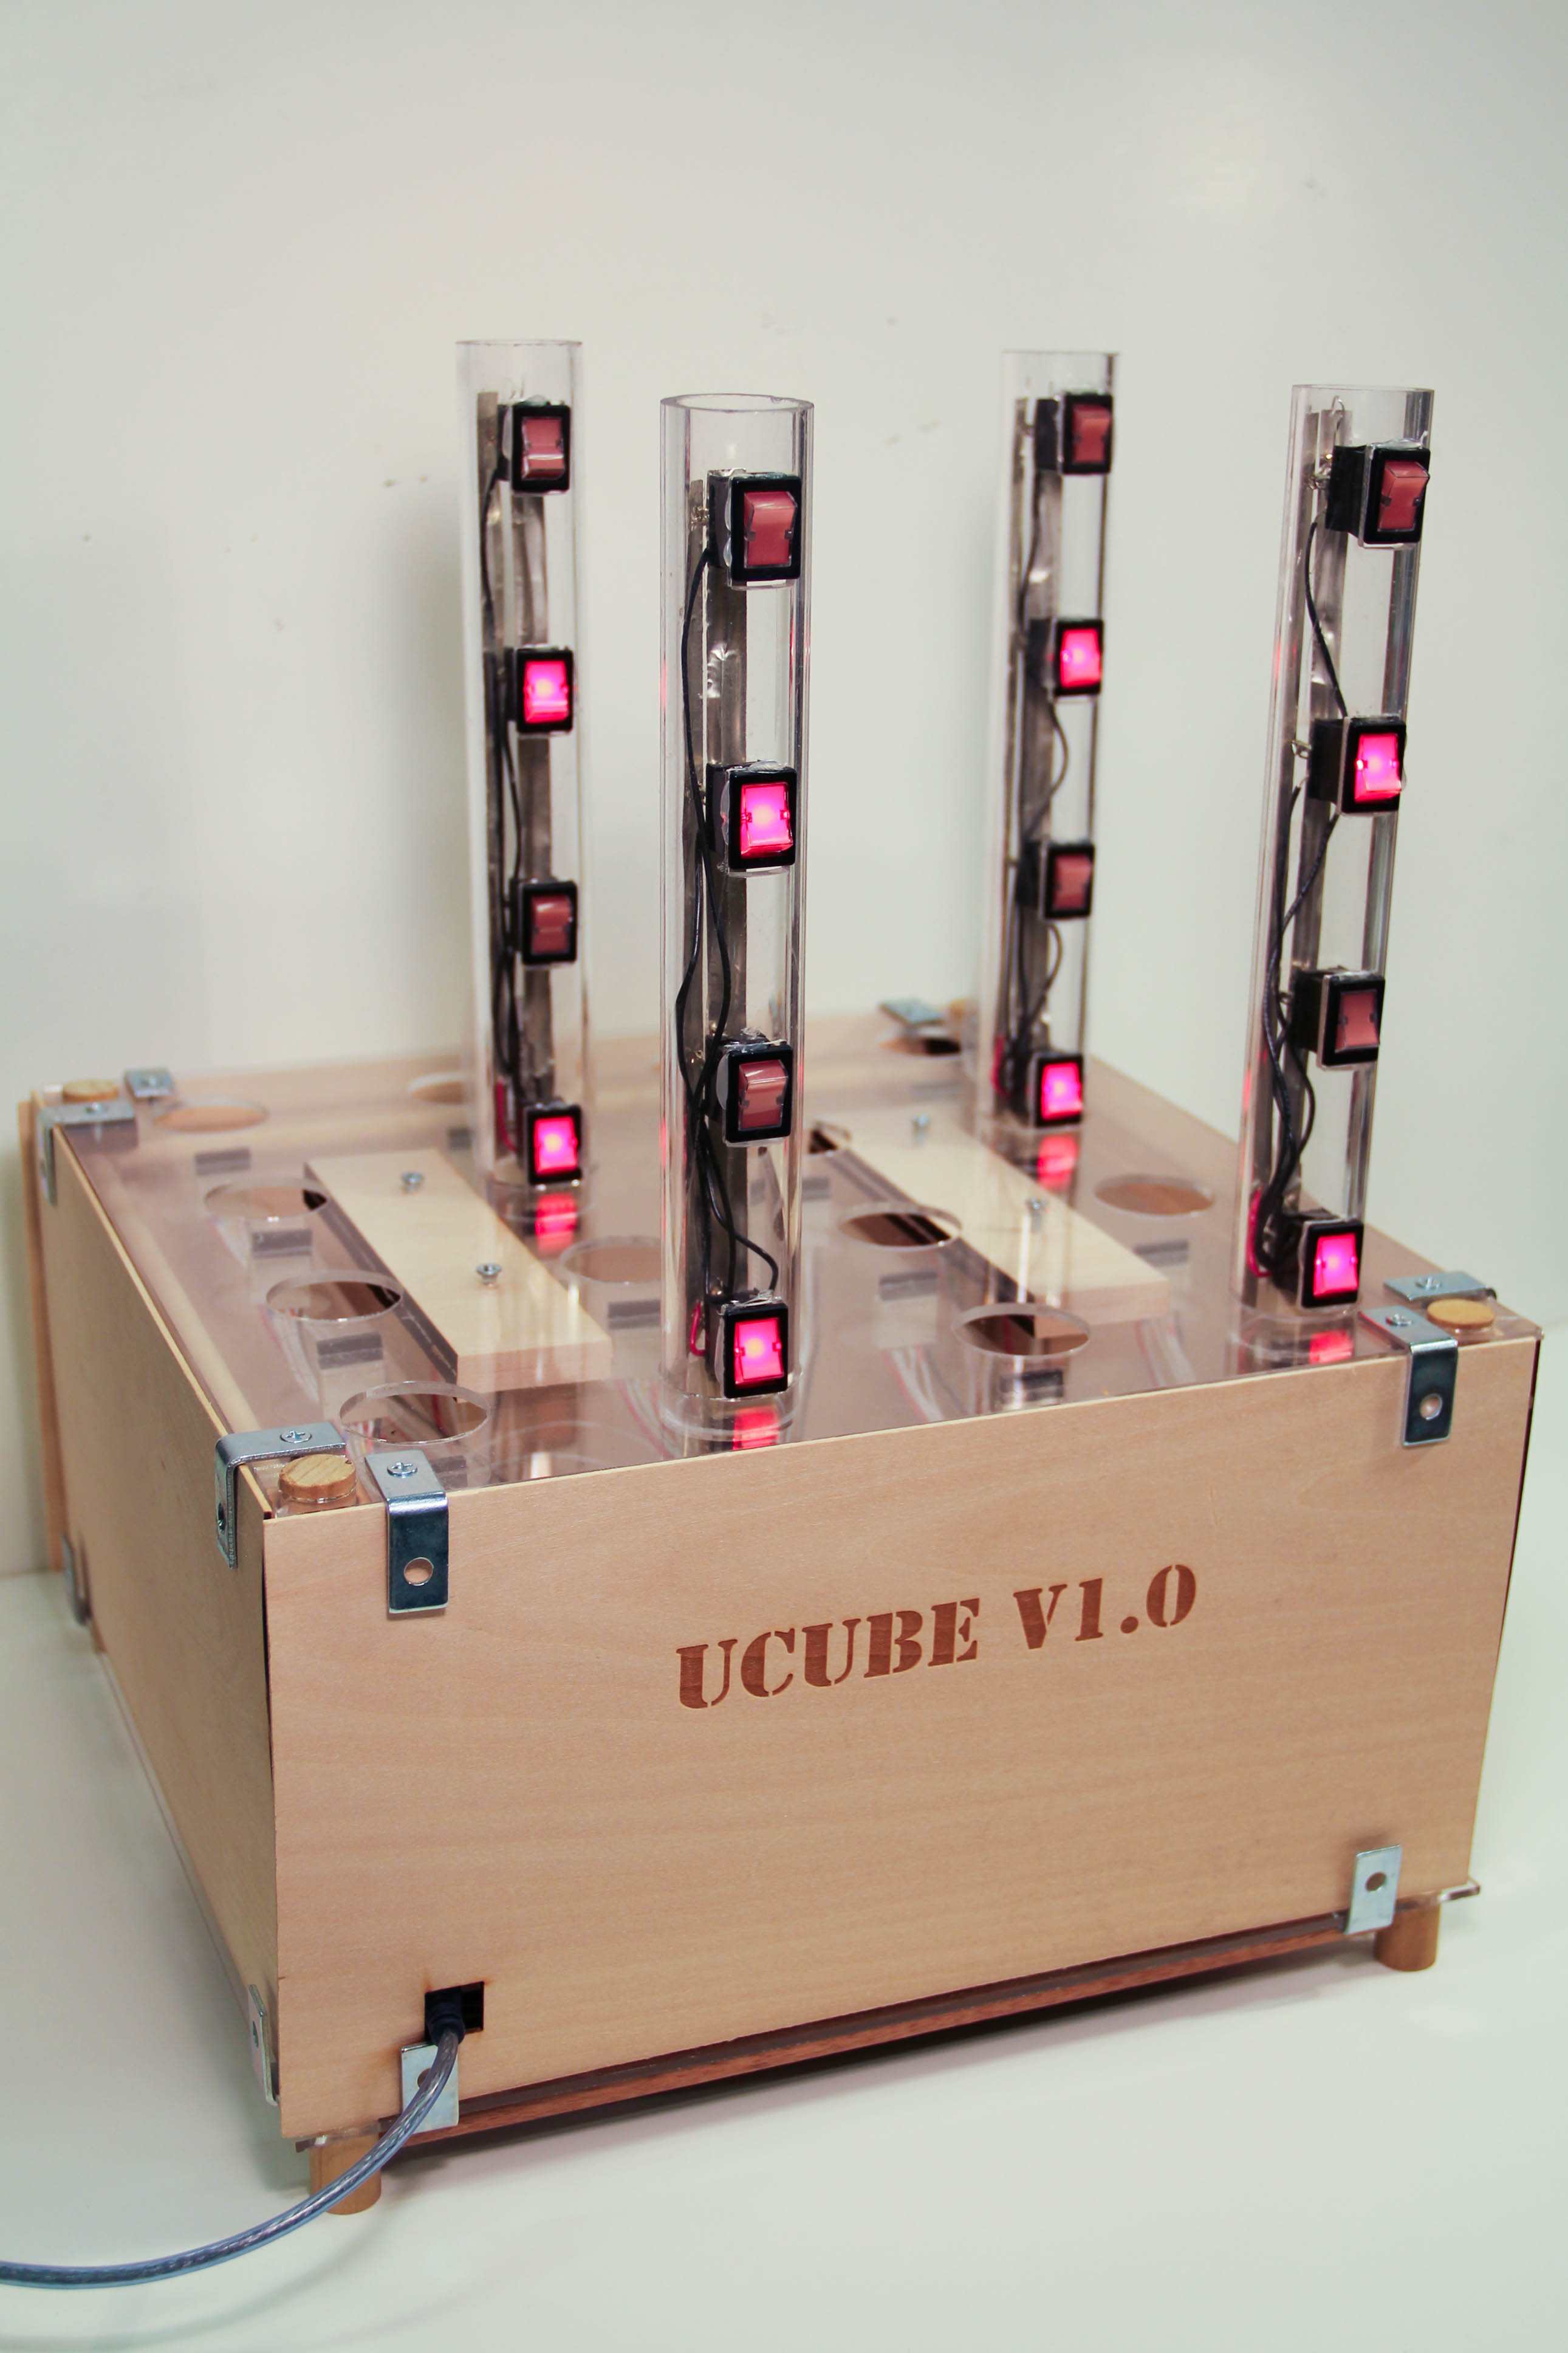
\includegraphics[width=.35\linewidth]{images/UCube-2}&
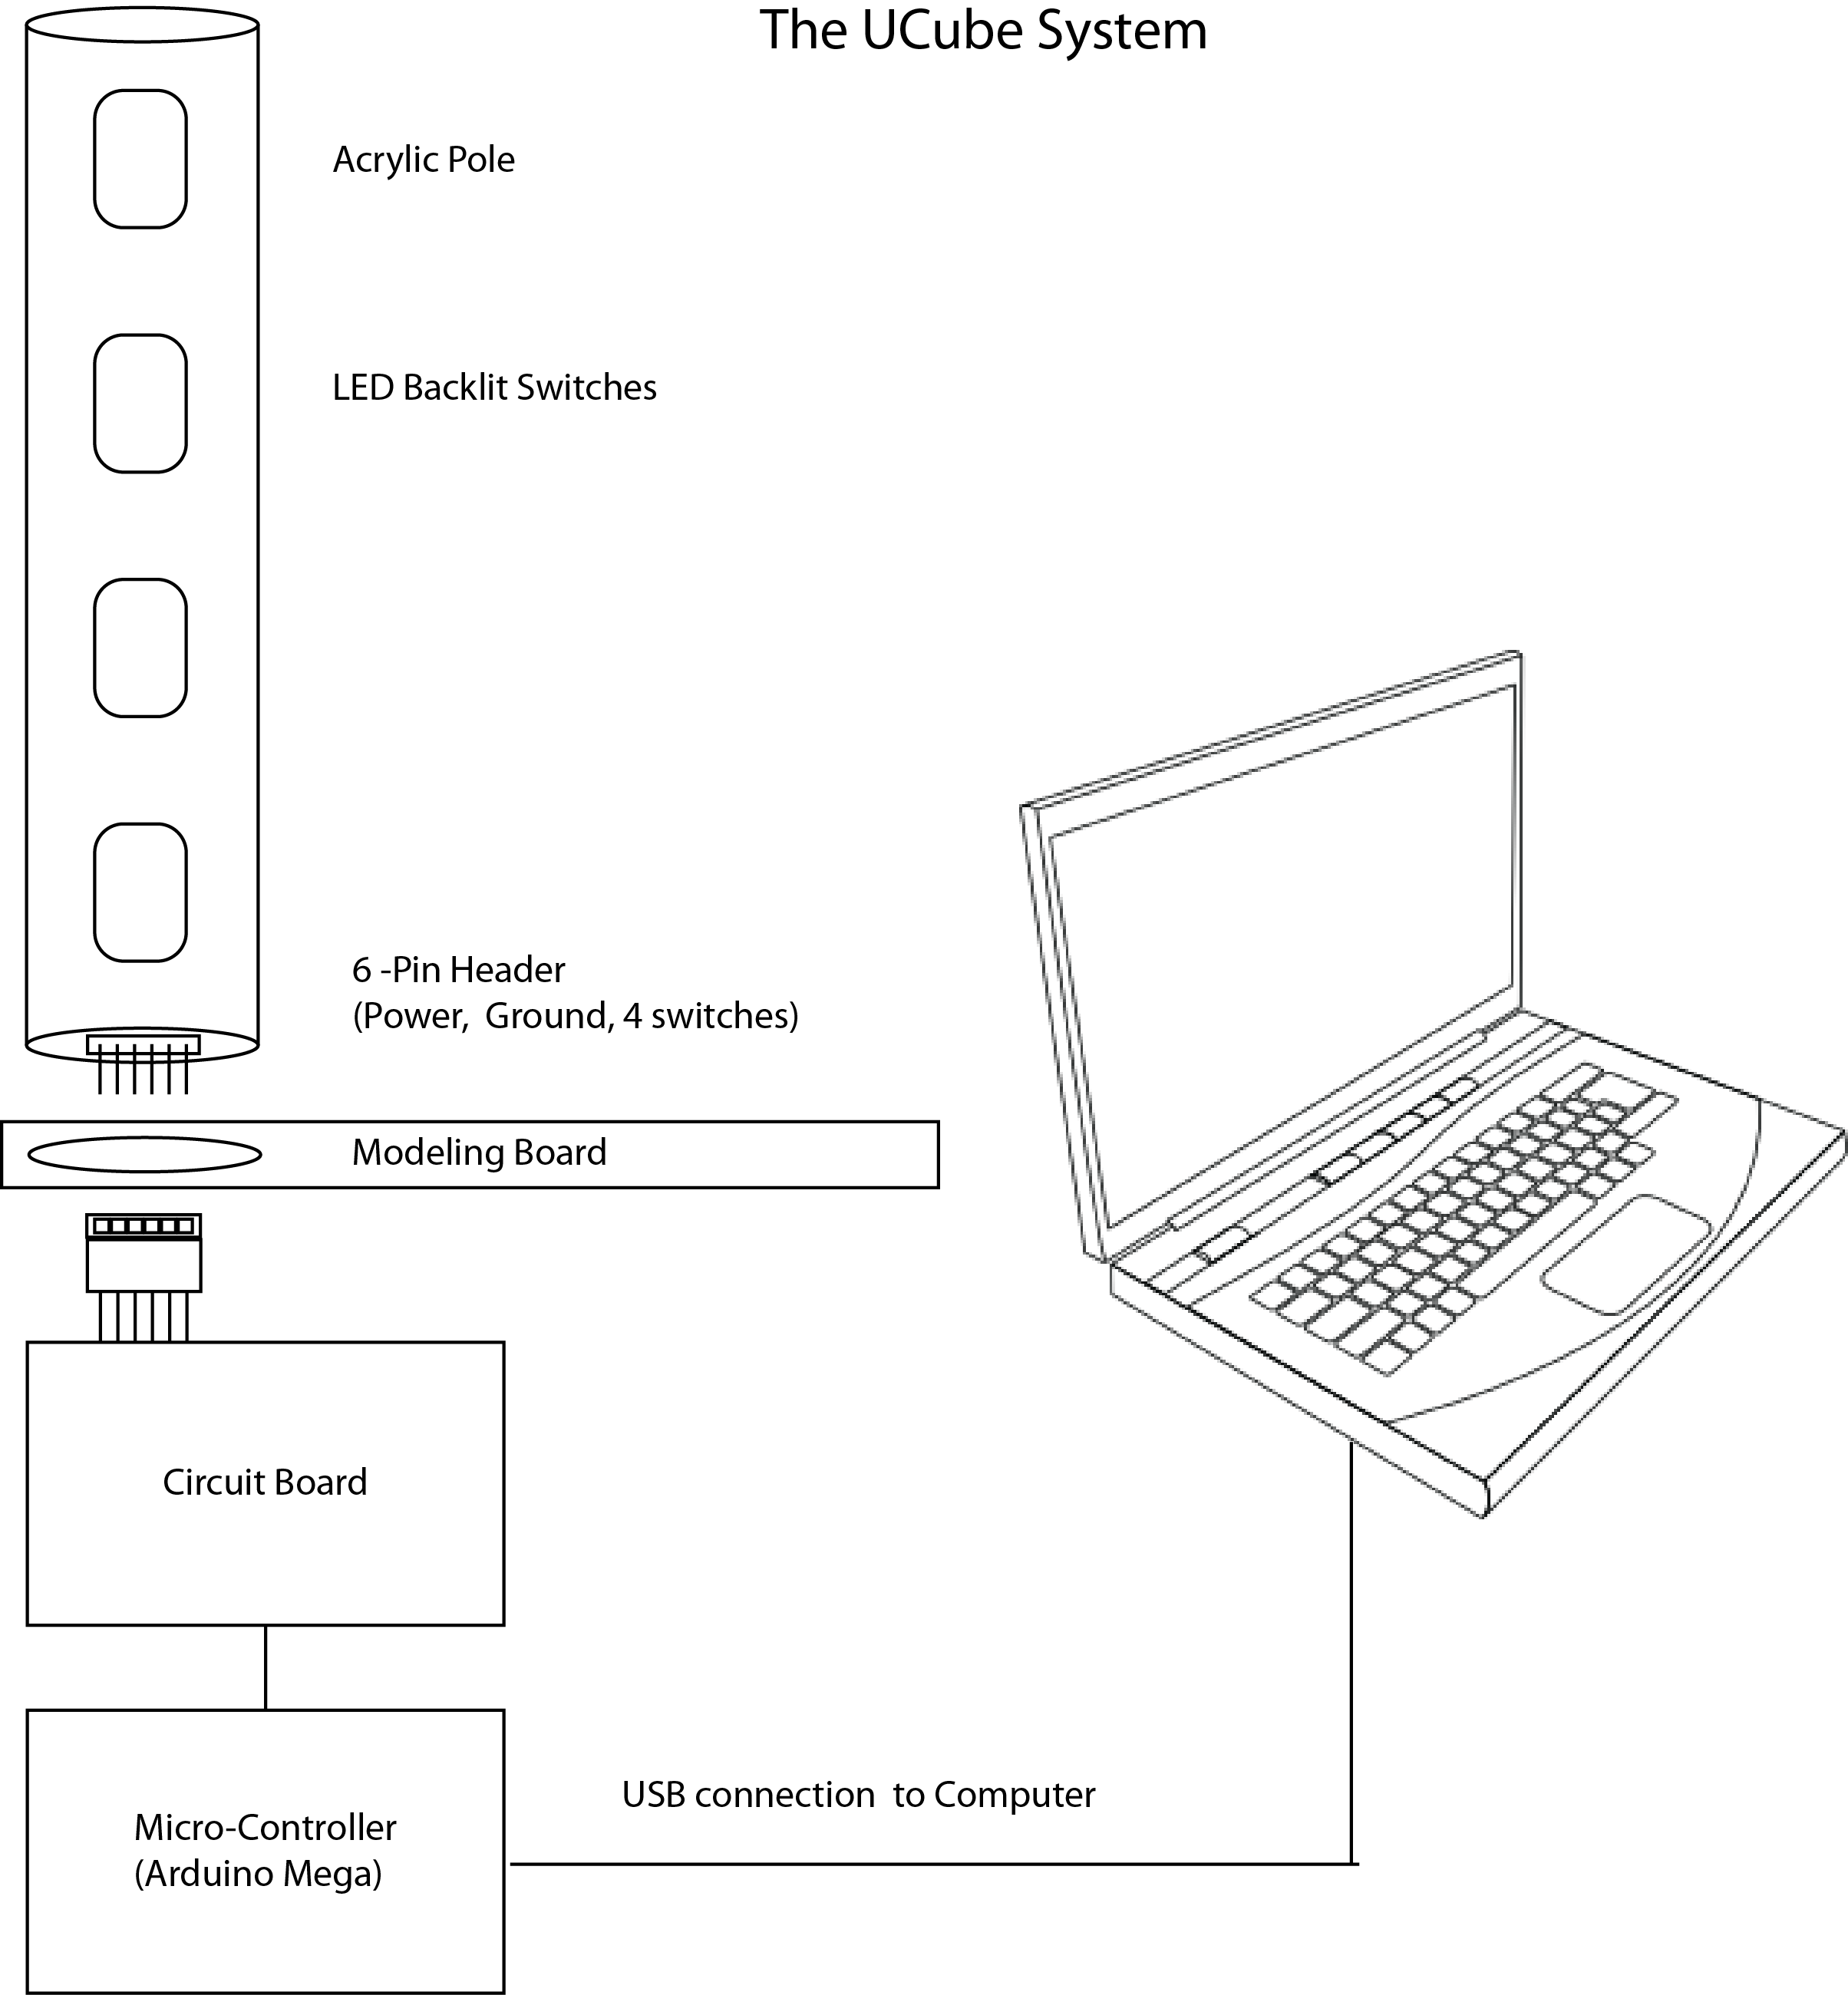
\includegraphics[width=.48\linewidth]{images/ucube_diagram}
\end{array}$
\end{center}
\caption{Left: The UCube device, with four towers and eight lit switches,
representing the eight vertices of a cube. Right: a schematic illustration of
the UCube hardware.}
\label{fig:cubev1}
\end{figure}

% We performed two separate studies using the first UCube interface with
% middle school children aged 11-14. The first (informal) study, detailed in
% \cite{Leduc-Mills:2011:UCD:1999030.1999039} had fourteen participants,
% consisting of five girls and nine boys, who were divided into six groups (five
% groups of two, one group of four). Participants were asked to model a sequence
% of five shapes of increasing complexity using the UCube along with the companion
% software. The target shapes were displayed on one half of a computer screen,
% while the UCube software showing the live model was displayed on the other half.
% The shapes were as follows:  a straight vertical line, a diagonal line, a cube,
% a triangular prism, and finally an irregular polyhedral object. No shape
% required more than four towers to complete, and shapes were always presented in
% the same order. Of the six groups who participated, four groups successfully
% modeled all five shapes, one group ran out of time after three shapes, and one
% group finished one shape. Sessions lasted between 17 and 30 minutes.


\begin{figure}[ht]
\begin{center}$
\begin{array}{cc}
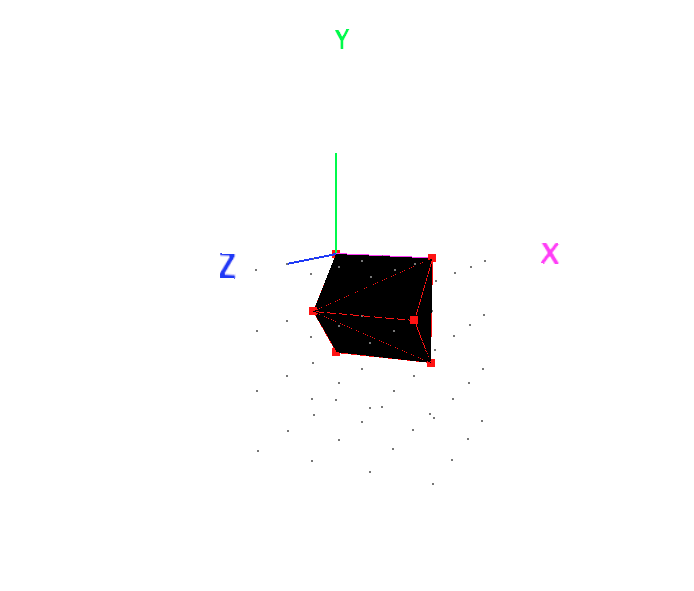
\includegraphics[width=.45\linewidth]{images/ucube1_software} &
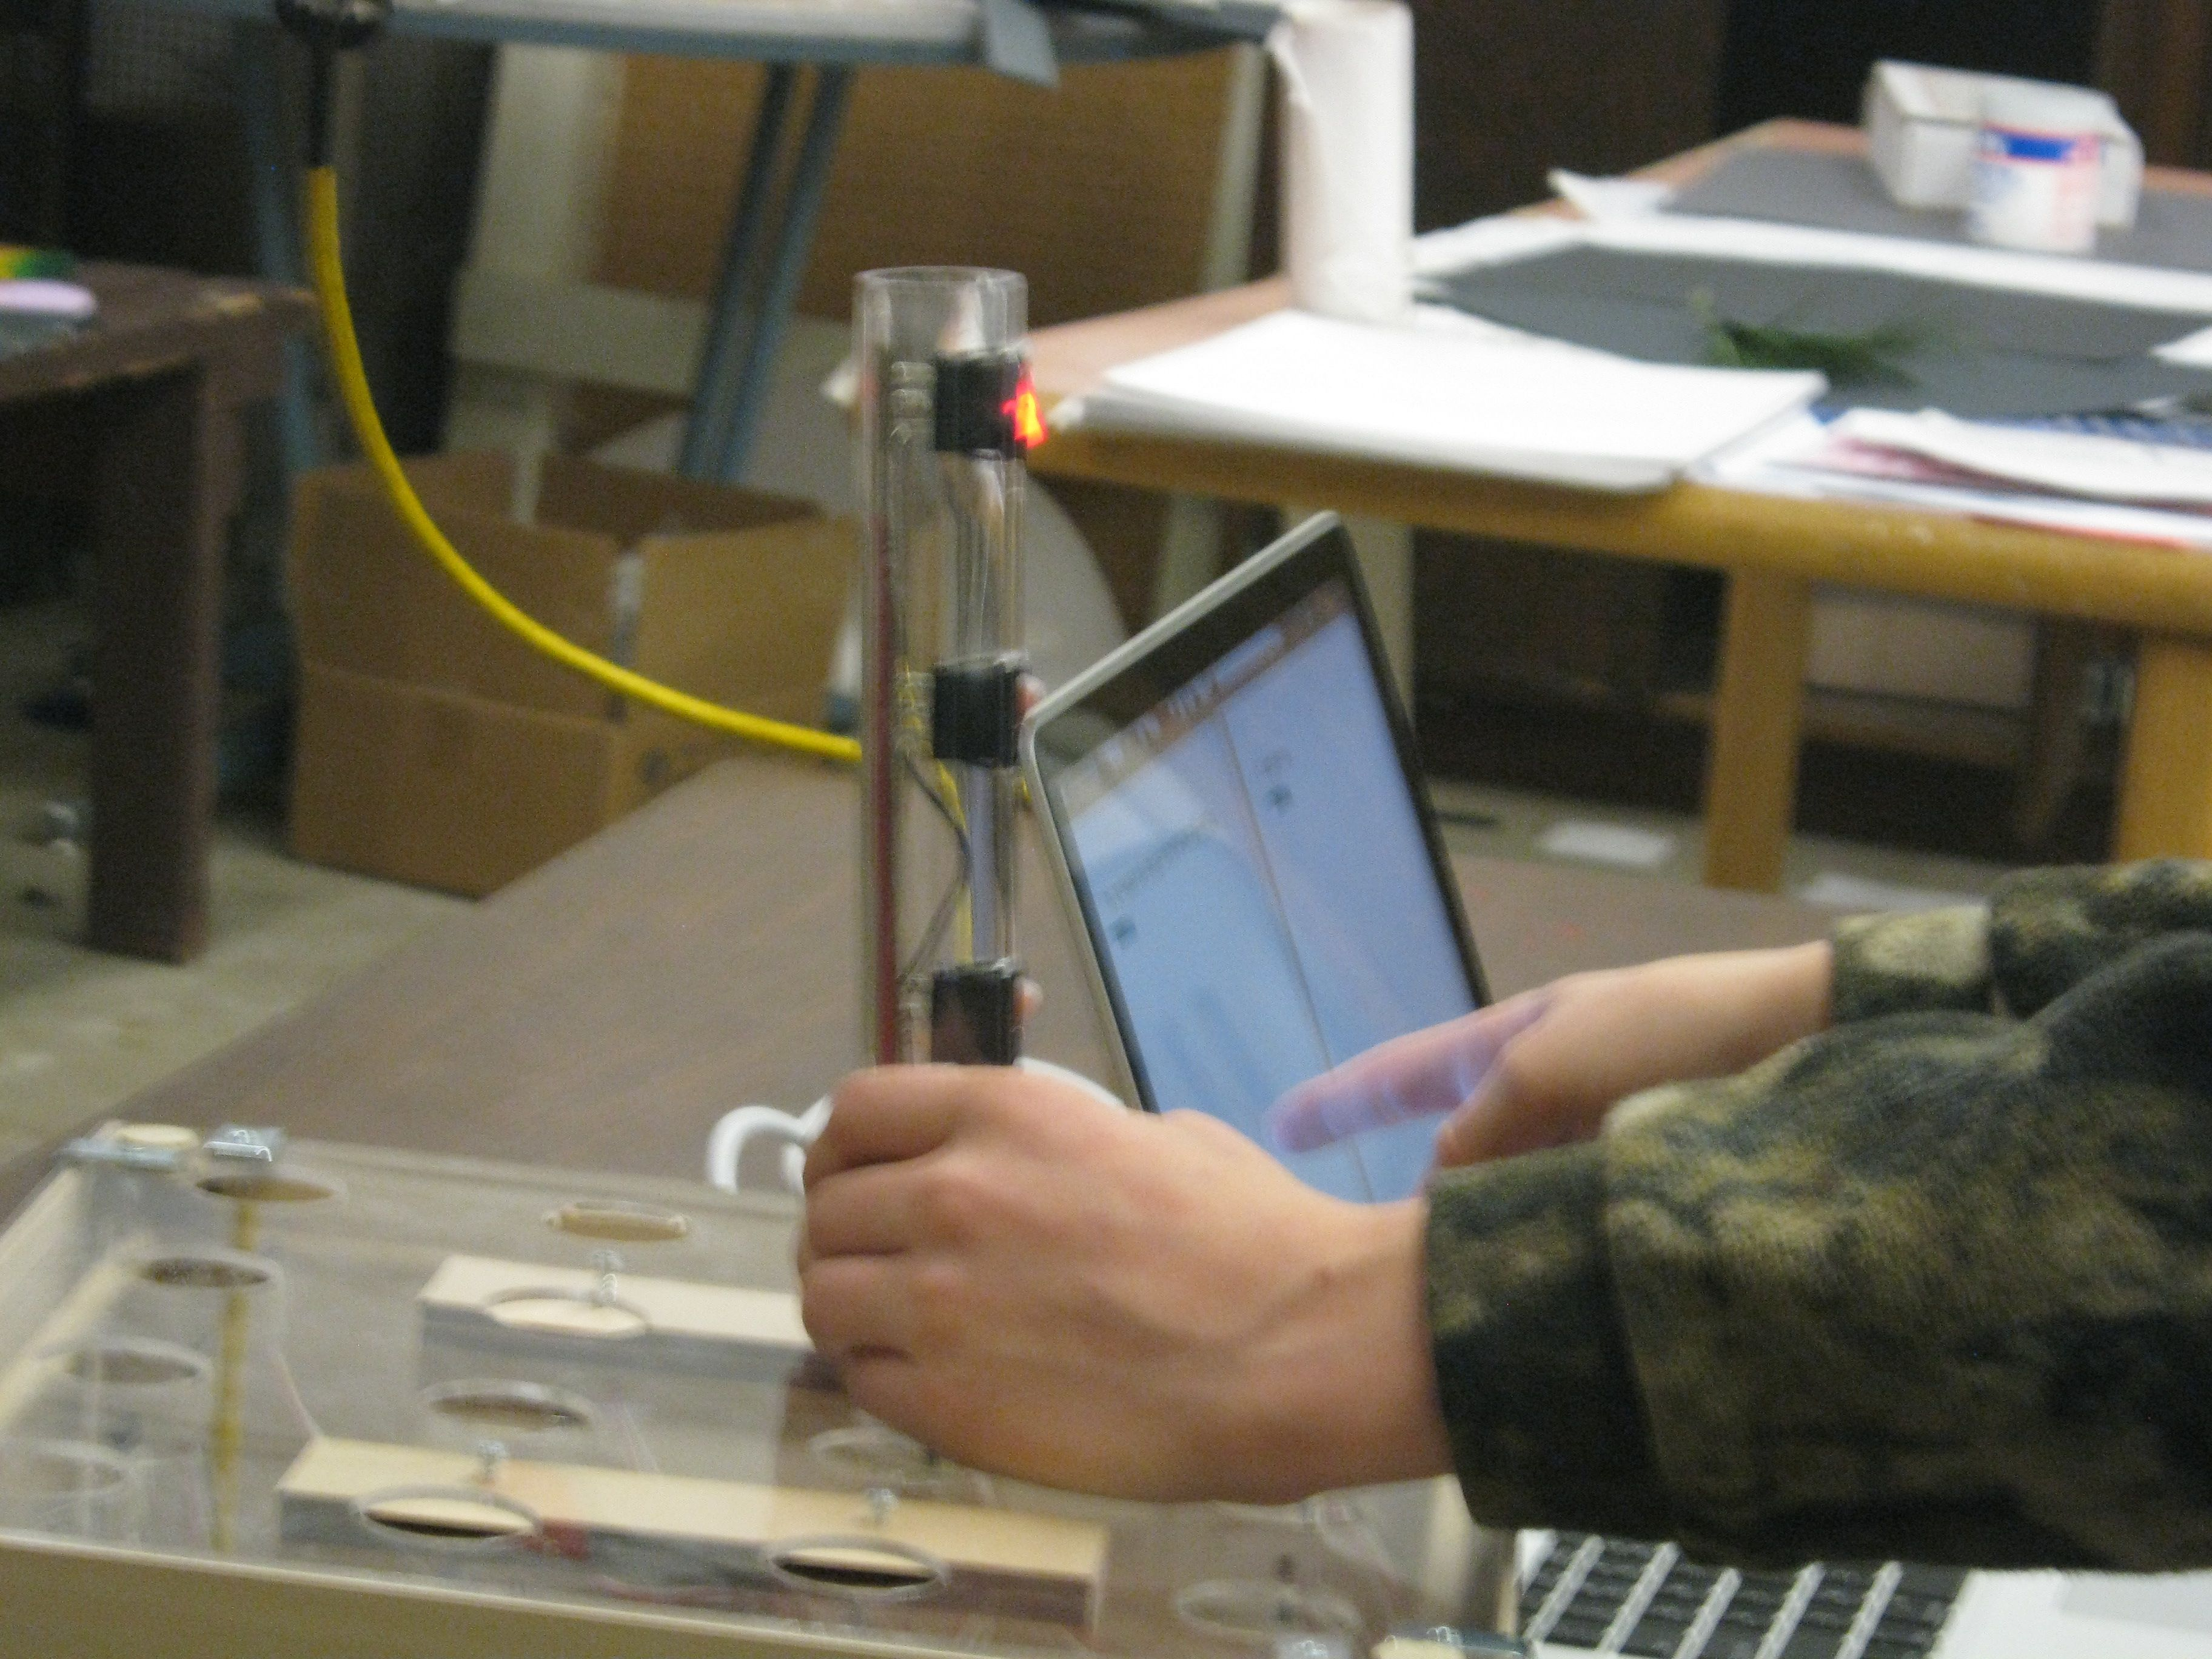
\includegraphics[width=.45\linewidth]{images/ucube1_user}
\end{array}$
\end{center}
\caption{Left: a screenshot of the UCube v1 software, showing the triangular
prism generated by performing the convex hull function on a set of 6 input
points. Right: A photograph of a middle-school student using the UCube. Here, the
student holds a tower in the platform and points simultaneously to the screen
representation of the selected point on the desktop computer.}
\label{fig:cubev2}
\end{figure}


% The second user study, from \cite{Leduc-Mills:2012:SSV:2307096.2307176},
% consisted of ten participants, eight boys and two girls, each of whom
% participated individually in two separate exercises. The first exercise was a
% modeling task, whereby the participant was handed a series of 3D-printed shapes
% and asked to recreate them on the UCube interface. The five physical models
% presented were: a cube, a tetrahedron, a diamond, a �house� (a cube with a
% pyramid on top), and a complex irregular polyhedron. The results were promising:
% overall, 21 of 50 shapes were completed from memory, 12 of 50 were completed
% while holding the shape, and a further 8 of 50 were completed with the aid of
% the UCube software, for a total of 41 out of 50 shapes modeled successfully
% (82\%). Of the nine missed shapes, seven were of the same shape, the complex
% polyhedron. The remaining two misses were from the same participant, who ran out
% of time before completion.
% 
% The second task was a matching task whereby participants were instructed to face
% away from the UCube while the facilitator modeled a set of lights on the UCube
% corresponding to one shape among a set of nine physical models laid out on the
% table next to the UCube. Once the lights on the UCube were set up, the
% participant was instructed to turn around, and indicate which physical object
% they thought the set of lights on the UCube corresponded to. Of the nine shapes,
% the participants were asked to match five of them (a cube, a triangular prism, a
% parallelogram, an elongated hexagon, and a trapezoid). Thus, only the cube was
% presented in both the matching and modeling exercises. Out of 50 matching tasks
% (5 per participant), 0 tasks resulted in the incorrect match being selected, and
% most matches were made in under 20 seconds, an encouraging result that points to
% the ability of children (of this age) to recognize convex hulls from a set of
% illuminated points.

% from IDC 2011 paper
As a first step in discussing the UCube's role in spatial design�and in
discussing the broader issue of children's three-dimensional design�this section
is devoted to a more thorough description of the UCube and its operation.
To begin with an overview, then: the UCube system is the combination of two
elements: the physical input device of ``towers'' placed on a board, and the
companion display software. These two systems work together to take the embodied
actions of the user and display corresponding points and shapes on the computer.
A sense of the scale of the device can be inferred from \autoref{fig:cubev2},
which shows a photograph of a middle-school student holding a newly-placed tower
in the UCube platform while pointing simultaneously at the desktop computer
screen beside it.
This photograph�which we will also return to in the discussion of pilot testing
in a later section�reflects the essential nature of interaction with the device:
points are designated in a spatial region provided by the platform, and then
represented in real time on the computer screen. Thus, the UCube promotes an
attention to the correspondence between the selected spatial points above the
platform and the (more abstract) representation on the computer screen.

\subsection{Hardware} 
The physical system for our first UCube prototype, as outlined earlier, consists
of a platform with a four-by-four grid of potential sites, each of which can
hold one tower with four switches, thus describing a 4x4x4 array of 64 potential
points.
The platform structure consists of three different horizontal ``layers''. The
top (or upper surface) layer has a four-by-four grid of circular holes, into
which the towers fit snugly. This layer of 1/4'' thick laser-cut clear acrylic
acts as a brace to hold the towers upright, and ensures that they are resistant
to being knocked over. The next layer down holds the headers, which allow the
towers to ``plug in'' and connect to the rest of the circuit. Wires from the
headers go down to the bottom layer, which holds the breadboarded circuit and
Arduino Mega microcontroller. The towers are made of transparent acrylic, the
side paneling of basswood. The towers were laser-cut in order to house the four
switches and corresponding circuitry elements. The switches are LED-backlit when
active, making it more apparent which points are active as well as giving a more
accessible ``gestalt'' of the shape being modeled. It also allows for some
potentially interesting applications in dimly-lit circumstances, such as
modeling constellations in a classroom or planetarium: in these situations, the
lights of the selected spatial points stand out especially vividly.

Each tower connects to the platform through a six-pin header (one pin each for
power, ground, and four switches). The switch connections are then routed
through a breadboard containing current limiting resistors for the LED switches
to pins on a microcontroller (an Arduino Mega\cite{ArduinoMega}).
The Arduino is then able to communicate (via asynchronous serial communication)
the active switches (and corresponding coordinates) to the computer through a
USB cable. \autoref{fig:cubev1}(right) depicts a schematic diagram of the UCube
hardware.

% \subsection{Software}
% 
% The UCube makes use of the Processing\cite{Processing} framework to read in
% the active coordinates from the Arduino microcontroller connected to the
% platform; the software then displays these as larger red points on a grid of
% grey dots. Users can rotate the grid along any axis by clicking and dragging
% with the mouse. In our current early prototype, there are only two buttons on
% the user interface: (i) an �export� button, responsible for taking the current
% set of active points and exporting them into "STL" file format (suitable for 3D
% printers), and (ii) a �mode� button which toggles between showing just the red
% dots as points and filling in an area (defined by a convex hull algorithm) to
% give a sense of shape.
% The software interface is intentionally minimal in order to encourage the user
% to focus on the physical interaction. We felt it was crucial not to fall into
% the trap of making another software tool for experts, so the main purpose of the
% software is to act as an aid�a means to cognitively clarify and confirm the
% user's intentions. Although it is likely that we will extend the software
% somewhat in future iterations, our goal is to support the physical experience of
% specifying a three-dimensional object, and not to add functionality beyond what
% is necessary or helpful to that end.

% \subsection{A Sample UCube Scenario}
% As a sample scenario, imagine that we wish to create a triangular prism solid
% employing the UCube. We can begin this process by selecting three points to form
% a triangle, as shown in Figure 6; then, by placing two more towers and creating
% the same triangular shape "shifted over" by two units (Figure 7) we create the
% entire prism. Naturally, there might be many alternative pathways to forming the
% same eventual shape: for example, we might begin by placing four (or more)
% towers in the platform, and then experiment or fiddle with the chosen lights to
% approach the eventual goal of creating our prism. Alternatively, we might begin
% without any towers in the device at all: by placing our hands or fingers above
% the device, roughly indicating where the prism should be, we might then use our
% imagined locations as "guides", helping us to place the necessary towers in the
% platform and select the correct lights for the vertices of the prism.
% In any event, having designed the prism using the UCube platform, and having
% checked that it looks like the correct shape on the computer screen, the final
% step is to export the shape into a format suitable for 3D printer output. The
% UCube software, as noted earlier, includes a feature for doing just this; and
% finally, we print out the prism, as shown in Figure 8.
% Figure 6. The first step in constructing our triangular prism: here, we create a
% planar triangular shape toward the left side of the platform, and can see the
% resulting shape on the computer screen shown at right.
% Figure 7. Completing the triangular prism. Here, we have added a second
% ("shifted") version of our original triangle to produce the six vertices needed
% to form the prism.

\subsection{Limitations}
It will probably not have escaped the reader's notice that the UCube, as a
three-dimensional modeling device, has significant limitations. To take the most
glaring of these: the user can only model those shapes whose vertices are among
the sixty-four locations accessible from the device. Moreover, those available
locations are evenly spaced in the form of a three-dimensional grid, or lattice;
thus, there are numerous simple-but-interesting shapes (such as the regular
dodecahedron, composed of regular pentagonal faces) that cannot be designed in
the current version of the UCube. Likewise, shapes with curved surfaces (such as
a cylinder), demanding at the very least a high resolution of accessible points,
could not be modeled in the current UCube. We will return to these issues in the
final section of the paper, in the discussion of ongoing and future work.



\section{SnapCAD}

\begin{figure}[ht] \begin{center}$
\begin{array}{cc}
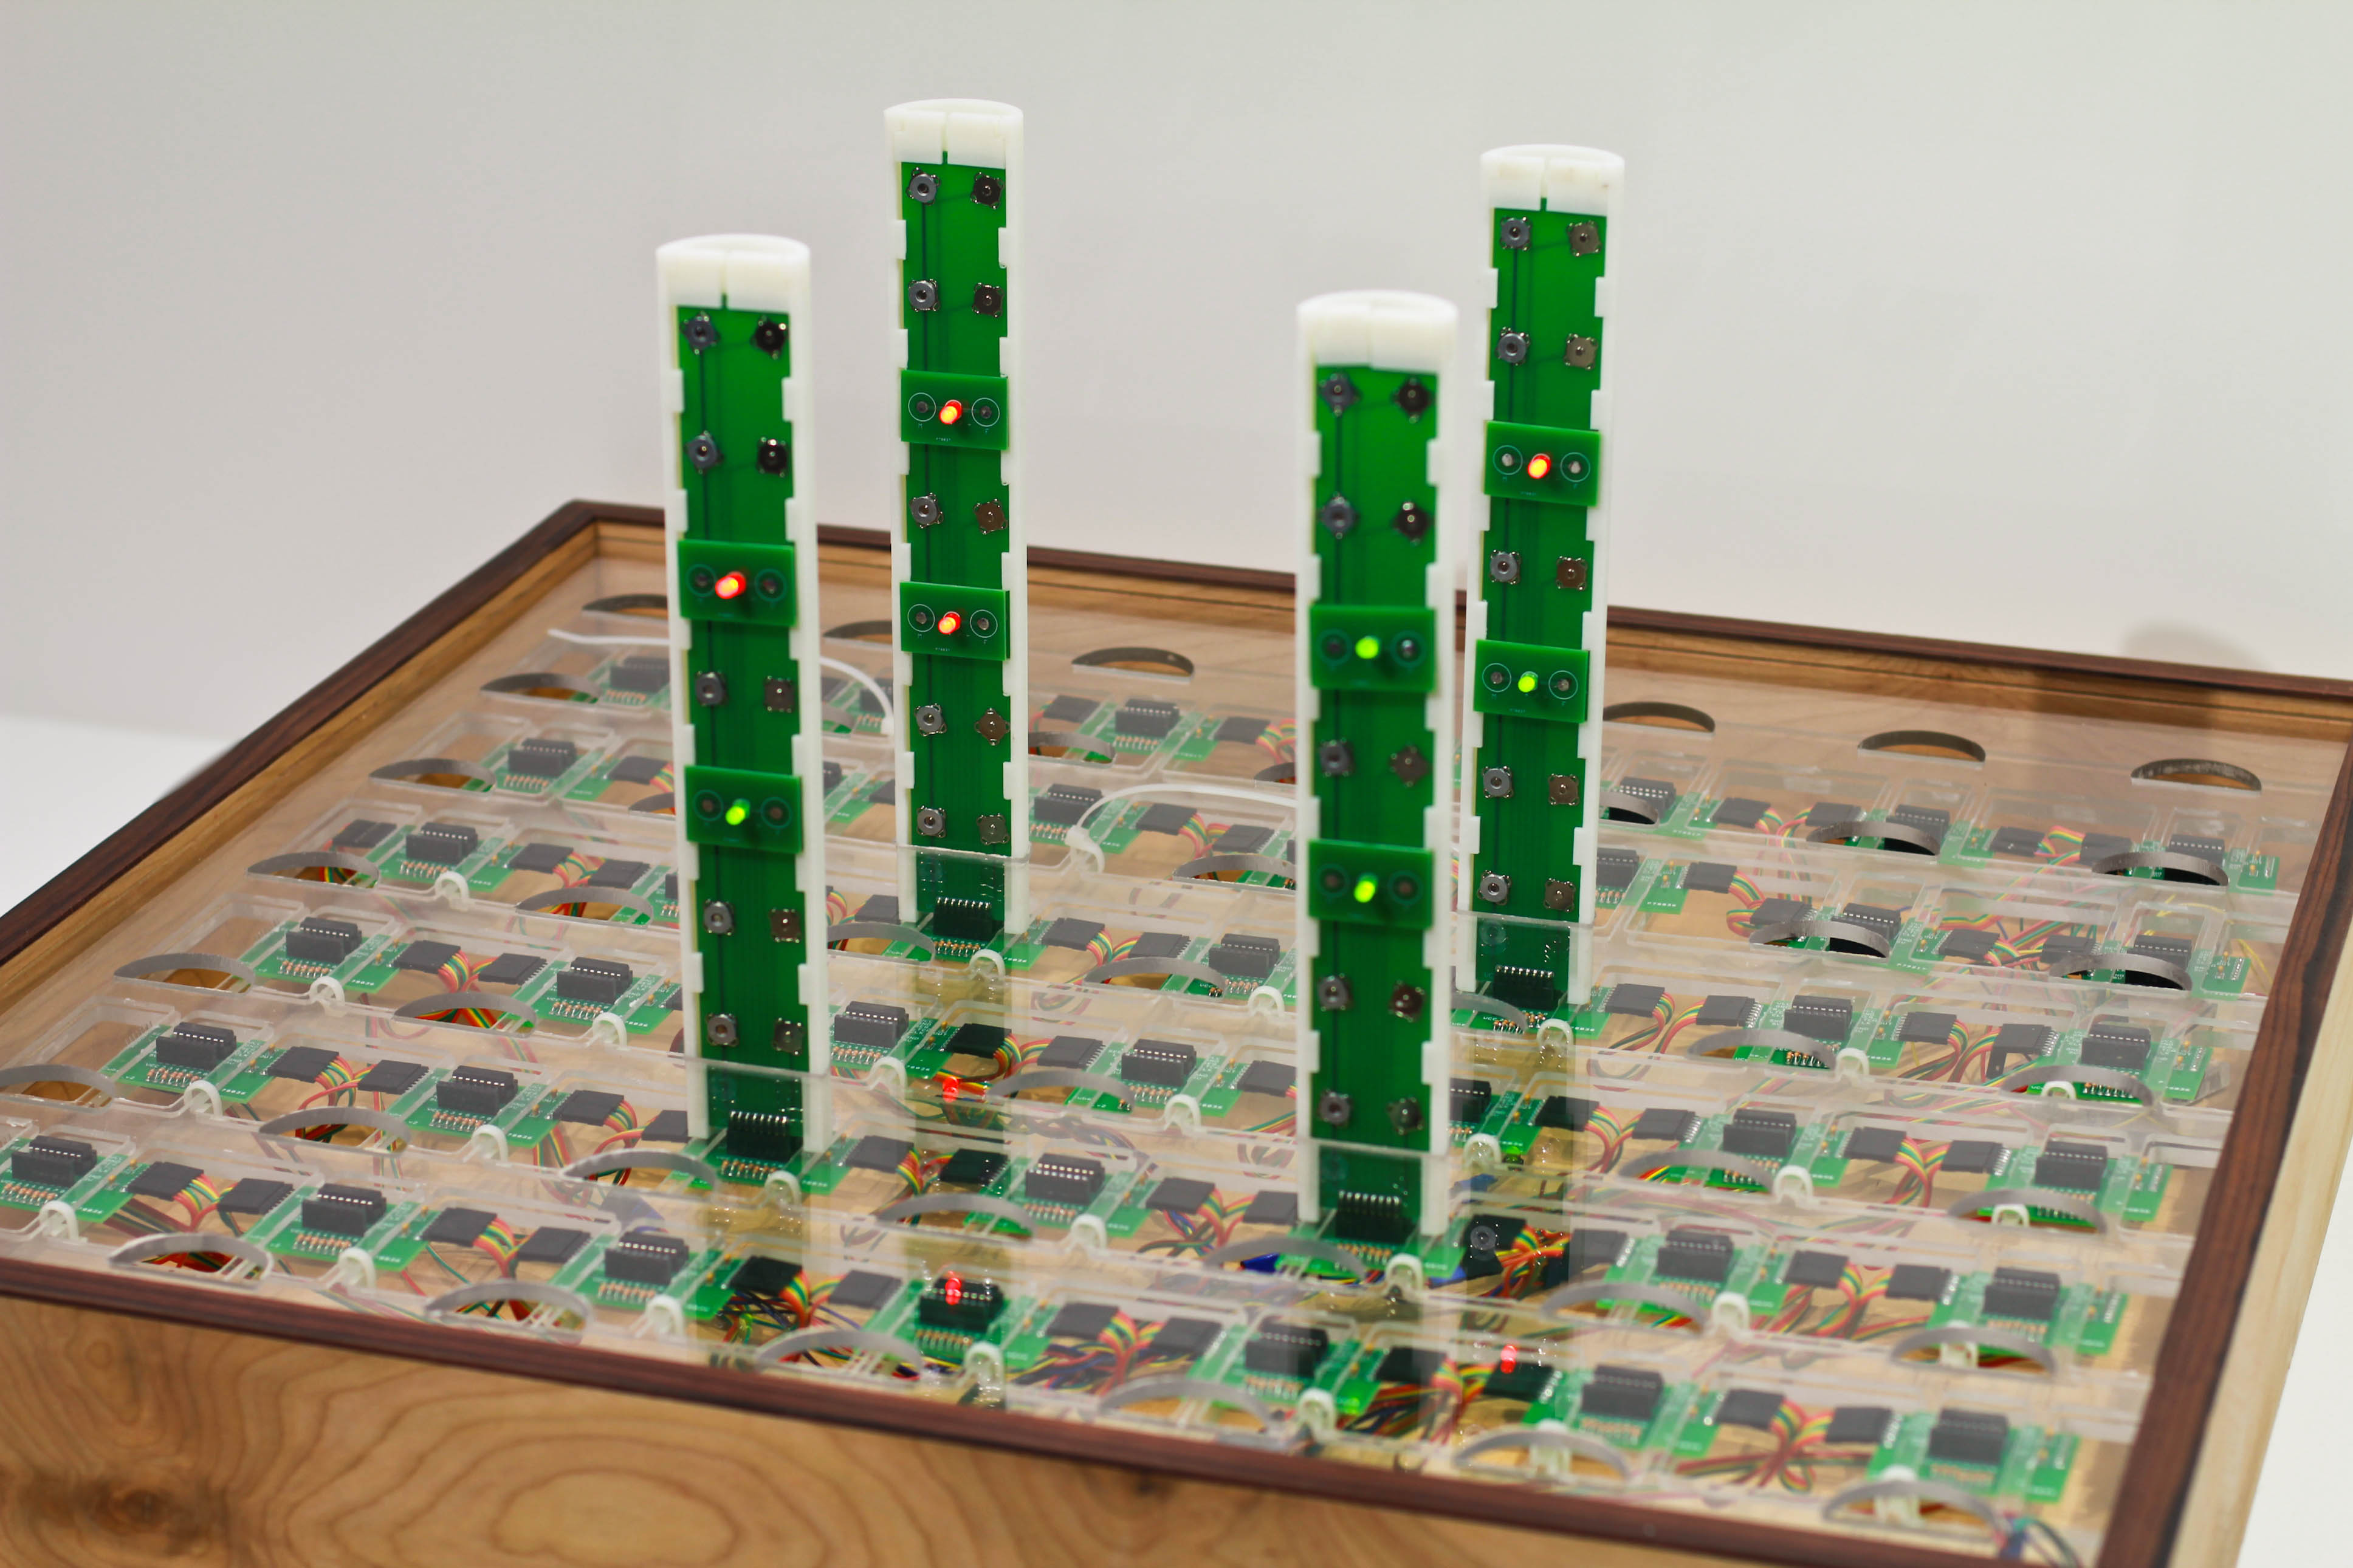
\includegraphics[width=.45\linewidth]{images/BeatriceFinal-2} & 
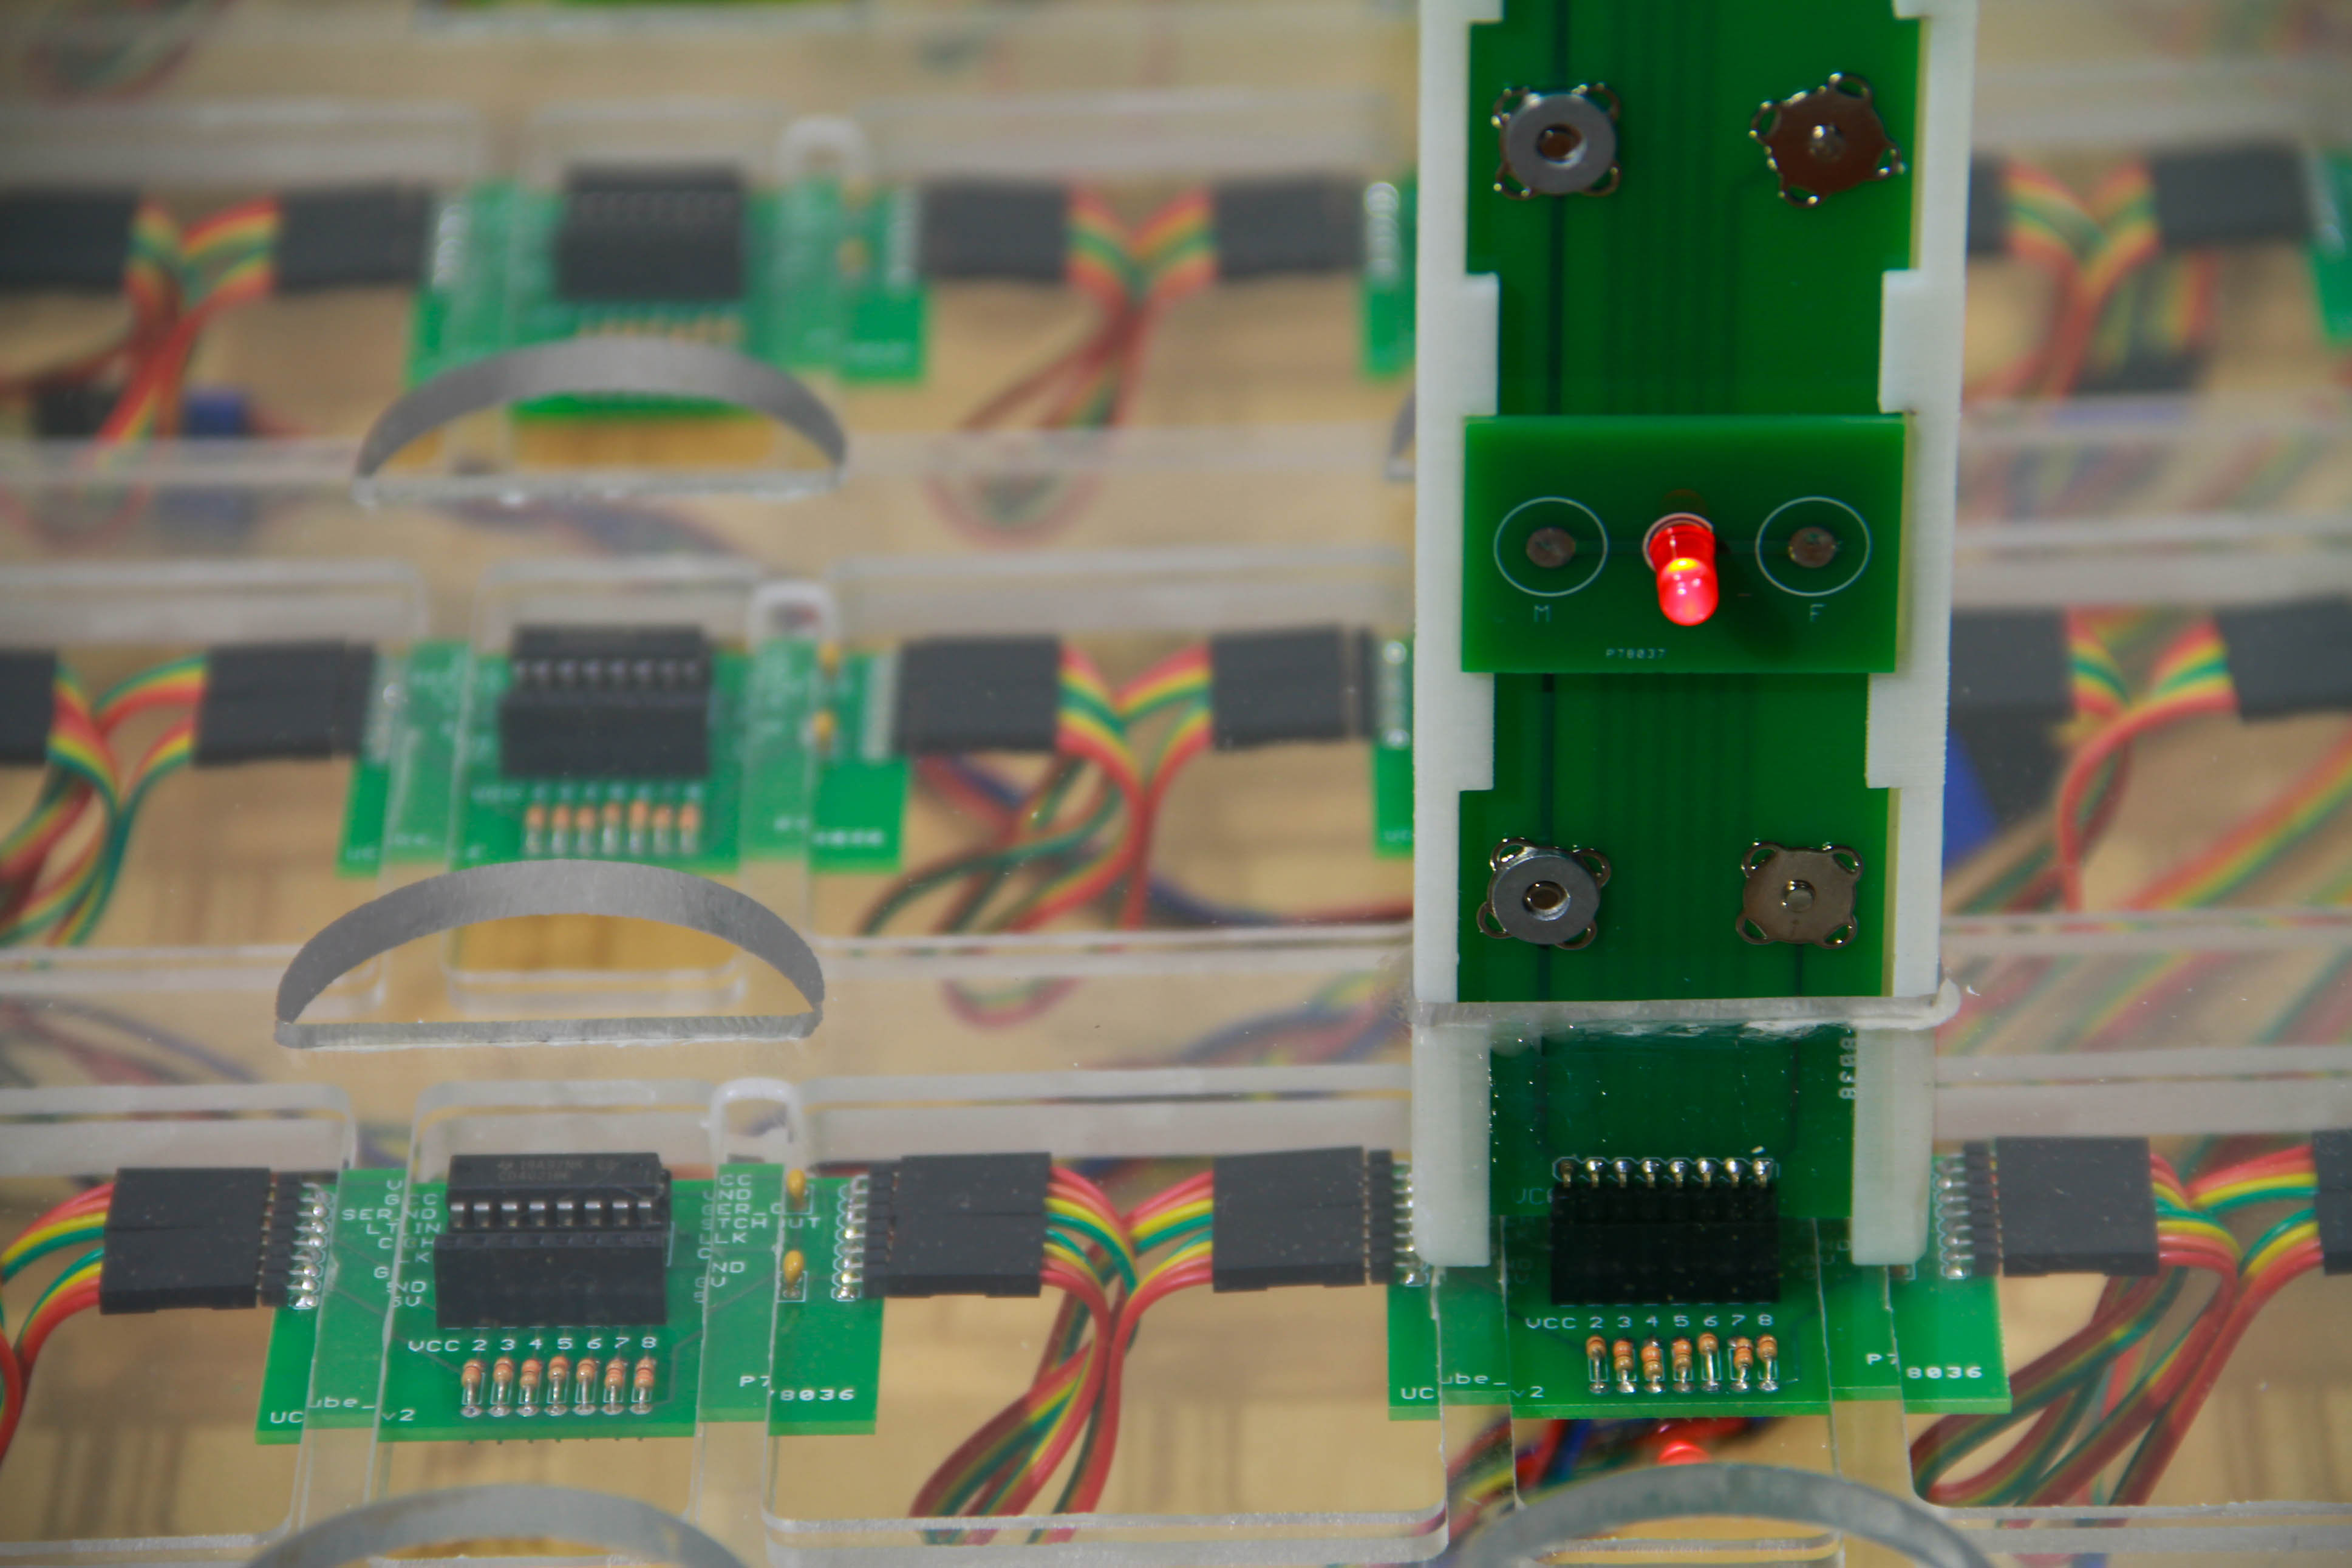
\includegraphics[width=.45\linewidth]{images/BeatriceFinal-14}
\end{array}$
\end{center}
\caption{
Left: the SnapCAD interface, showing the hardware configuration corresponding to
the picture below in \autoref{fig:ucubev22}. Right: a detail of the SnapCAD
hardware - the PCB tower is housed in a 3D-printed shell, which plugs into a
shift-register board. The LED boards snap on to the towers via magnetic snaps.}
\label{fig:ucubev21}
\end{figure}

Based on the feedback from these two user studies, a second, more powerful
instantiation of the ideas from the UCube has been created. SnapCAD (formerly
known as UCube v2) consists of a total input space of 7x7x7 points, forming 343
distinct coordinates. In our user studies with UCube v1, we noticed that users
often encountered initial difficulties when required to `find a middle' in the
shape they were attempting to model, given an even number of total grid spaces.
For example, to model a pyramid on on a 4x4x4 grid, one needs to construct a 3x3
subset of the 4x4 grid, using the middle point within the 3x3 set as the top of
the pyramid. This influenced our decision to create an odd-numbered layout,
creating a more `natural' middle point in the hardware. The greater number of
inputs vastly increases the expressive potential of SnapCAD (compared to the
UCube) while still maintaining a manageable interface.
Working on the scale of multiple hundreds of inputs necessitated the design of
custom circuit boards to relay information effectively to the microcontroller.
This change in scale also meant rewriting most of the modeling software to
effectively handle the greater expressiveness of the physical system.



\begin{figure}[ht] \begin{center}$
\begin{array}{cc}
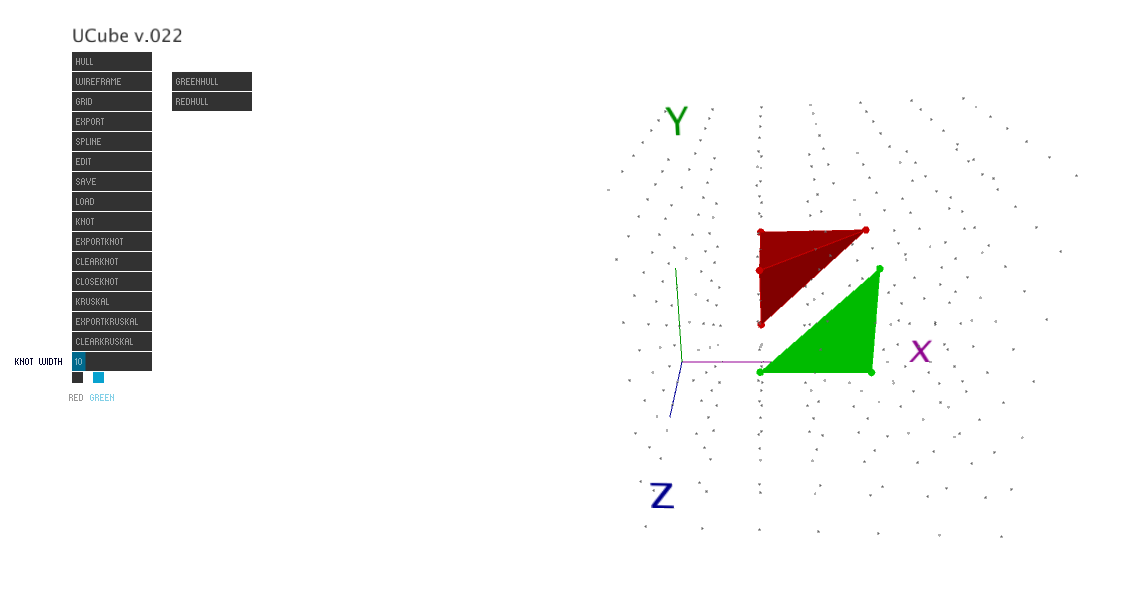
\includegraphics[width=.45\linewidth]{images/twoHulls} &
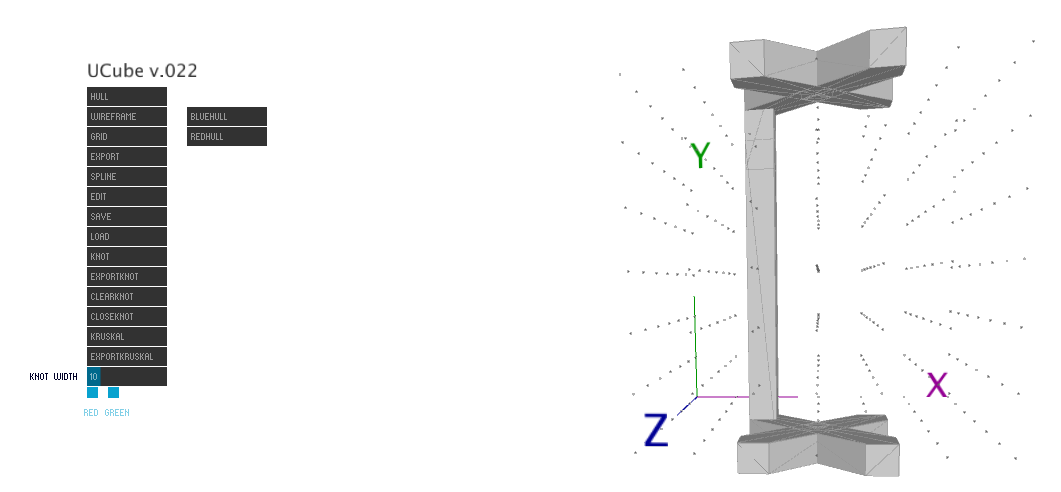
\includegraphics[width=.45\linewidth]{images/mst}
\end{array}$
\end{center}
\caption{Left: The SnapCAD software showing two convex hulls of different
colors. Right: the SnapCAD software showing a minimal spanning tree model.}
\label{fig:ucubev22}
\end{figure}


The use of conductive, magnetic snaps along towers constructed of custom-printed
circuit board allow for more than one color of illumination, as different
colored LED boards can be snapped onto any socket on the tower.
This not only results in the ability to represent multiple shapes at once, but
for the SnapCAD to become a platform for all manner of multi-player interactions
(e.g. games, puzzles, shape matching contests), with each `player' assigned a
unique color. To this end, we have created a simple `3D Tic-Tac-Toe'
implementation on the SnapCAD. Additional changes to the software include
supporting multiple but separate convex hulls of different colors, the ability
to create and export shapes created from the minimal spanning tree of a set of
input points, and the ability to adjust the width of the segments in the
knot/path and minimal spanning tree modes.
The click-and-drag editing mode now includes the knot/sequential path and
minimal spanning tree modes as well as the convex hull mode. We also adjusted
the knot-forming algorithm to handle paths that cross or self-intersect, as well
as providing a `close knot' button to complete a circuit in a shape, allowing
for even more kinds of 3D-printable objects. While significant work has been
done to bring the UCube and SnapCAD to their current states, we believe not only
that there is room for additional improvements to be made, but that, as opposed
to focusing on a incremental but essentially similar interface as the subject of
a thesis, it is far more intellectually interesting to focus on a class of
objects that demonstrate multiple incarnations of a set of ideas.

% \section{Proposed Work: Technical Additions}
% The proposed work is in two sections: technical additions and
% evaluation. This section deals with the technical additions to the proposed
% devices: SnapCAD and PopCAD.
% 
% \subsection{SnapCAD}
% 
% With 343 potential points, a click-and-drag editing tool, and three separate
% modeling modes (convex hull, knot/path, and minimal spanning tree) the SnapCAD
% is capable of generating countless 3-dimensional forms.
% Although the potential for additional modeling tools is certainly a possibility
% (we have yet to experiment with curved surfaces, for instance) we believe that
% the multi-player `platform' aspects of the SnapCAD system are the most ripe for
% development. We already have two colors of LED boards, the ability to display
% two colors of convex hulls, and a 3D implementation of a two-player tic-tac-toe
% game. Displaying multiple colors of the path/knot and minimal spanning tree
% modes should be fairly straightforward to implement.
% We would also like to expand and change the colors currently being used - we
% currently use red and green LEDs, which would be problematic for anyone with
% red/green color blindness. We propose using three colors: red, blue, and purple.
% This not only allows for up to three-player interactions, but could help to
% solve a deeper problem: representing in hardware a node occupied by two players.
% Using an idiom where solely-occupied nodes are either blue or red, and a jointly
% occupied node is purple, we can then expand the types of games, puzzles, or
% modeling activities the SnapCAD system can support. Once these improvements are
% made we can expand the activities supported on SnapCAD. Developments include
% two-to-three player games like tic-tac-toe as well as games built
% off of the modeling capabilities of the SnapCAD (e.g. match the model generated
% by the computer, model a sequential path through a generated maze, place points
% on or interior to the convex hull until there are no more to be found). Colors
% can also be used for certain as-yet unexplored modeling operations (e.g., the
% set union, intersection, or difference). While some of these operations may
% prove difficult or even impossible, these are all avenues worth exploring, as
% they all point towards the extensibility and potential expressiveness of SnapCAD
% as a platform for future development.

\section{PopCAD}

Our motivations for creating alternative interfaces to the UCube and SnapCAD
stem from the desire to explore this intellectual space more generally; it is
far more interesting to discuss a \emph{class} of tangible interfaces for
scaffolding digital fabrication than it is to discuss a singular device. To this
end, we looked at some of the weaknesses of SnapCAD and towards technologies we
had yet to explore. While SnapCAD can admirably perform a number of modeling
tasks, it was always envisioned as one device amongst an `ecosystem' of next
generation fabrication tools. It has strengths, but obvious weaknesses as well;
in particular, the SnapCAD hardware was expensive to produce, and so would be a
difficult proposition for some schools or fab labs; it is also rather unwieldy
and unportable - it moderately heavy, fairly large, and has many separate pieces
that could break or go missing. Thus, an interface with cheaper and more
portable materials was desirable.

To address these issues we chose to build a pop-up book combining traditional
paper-crafts and paper-friendly electronics such as copper tape.
In recent years, revolutionary work has been done in combining electronics and
paper
crafting\cite{Qi:2010:EPE:1709886.1709909}\cite{Mellis:2013:MMC:2460625.2460638},
leading to new techniques and new uses for traditional materials. Paper is
inexpensive (especially when compared to circuit boards), light, and easily
portable, making it an ideal material choice for a device that would not suffer
the same limitations present in the SnapCAD. Although we often think of `paper'
as a rather static material, there are in fact many variations in the size,
weight, color, transparency, and composition of contemporary paper products. For
the initial prototype, we used a simple construction paper as it provided a
balance between strength and flexibility as well as having a consistency
well-suited to laser etching and cutting.
The pop-up book (named PopCAD) has a 3x3x3 array of 27 points which are evenly
spaced 3 inches apart on a 12'' x 18'' paper surface.
The book folds on a single center crease making the closed footprint of the book
roughly 12'' x 9''.

\begin{figure}[ht] \begin{center}$
\begin{array}{cc}
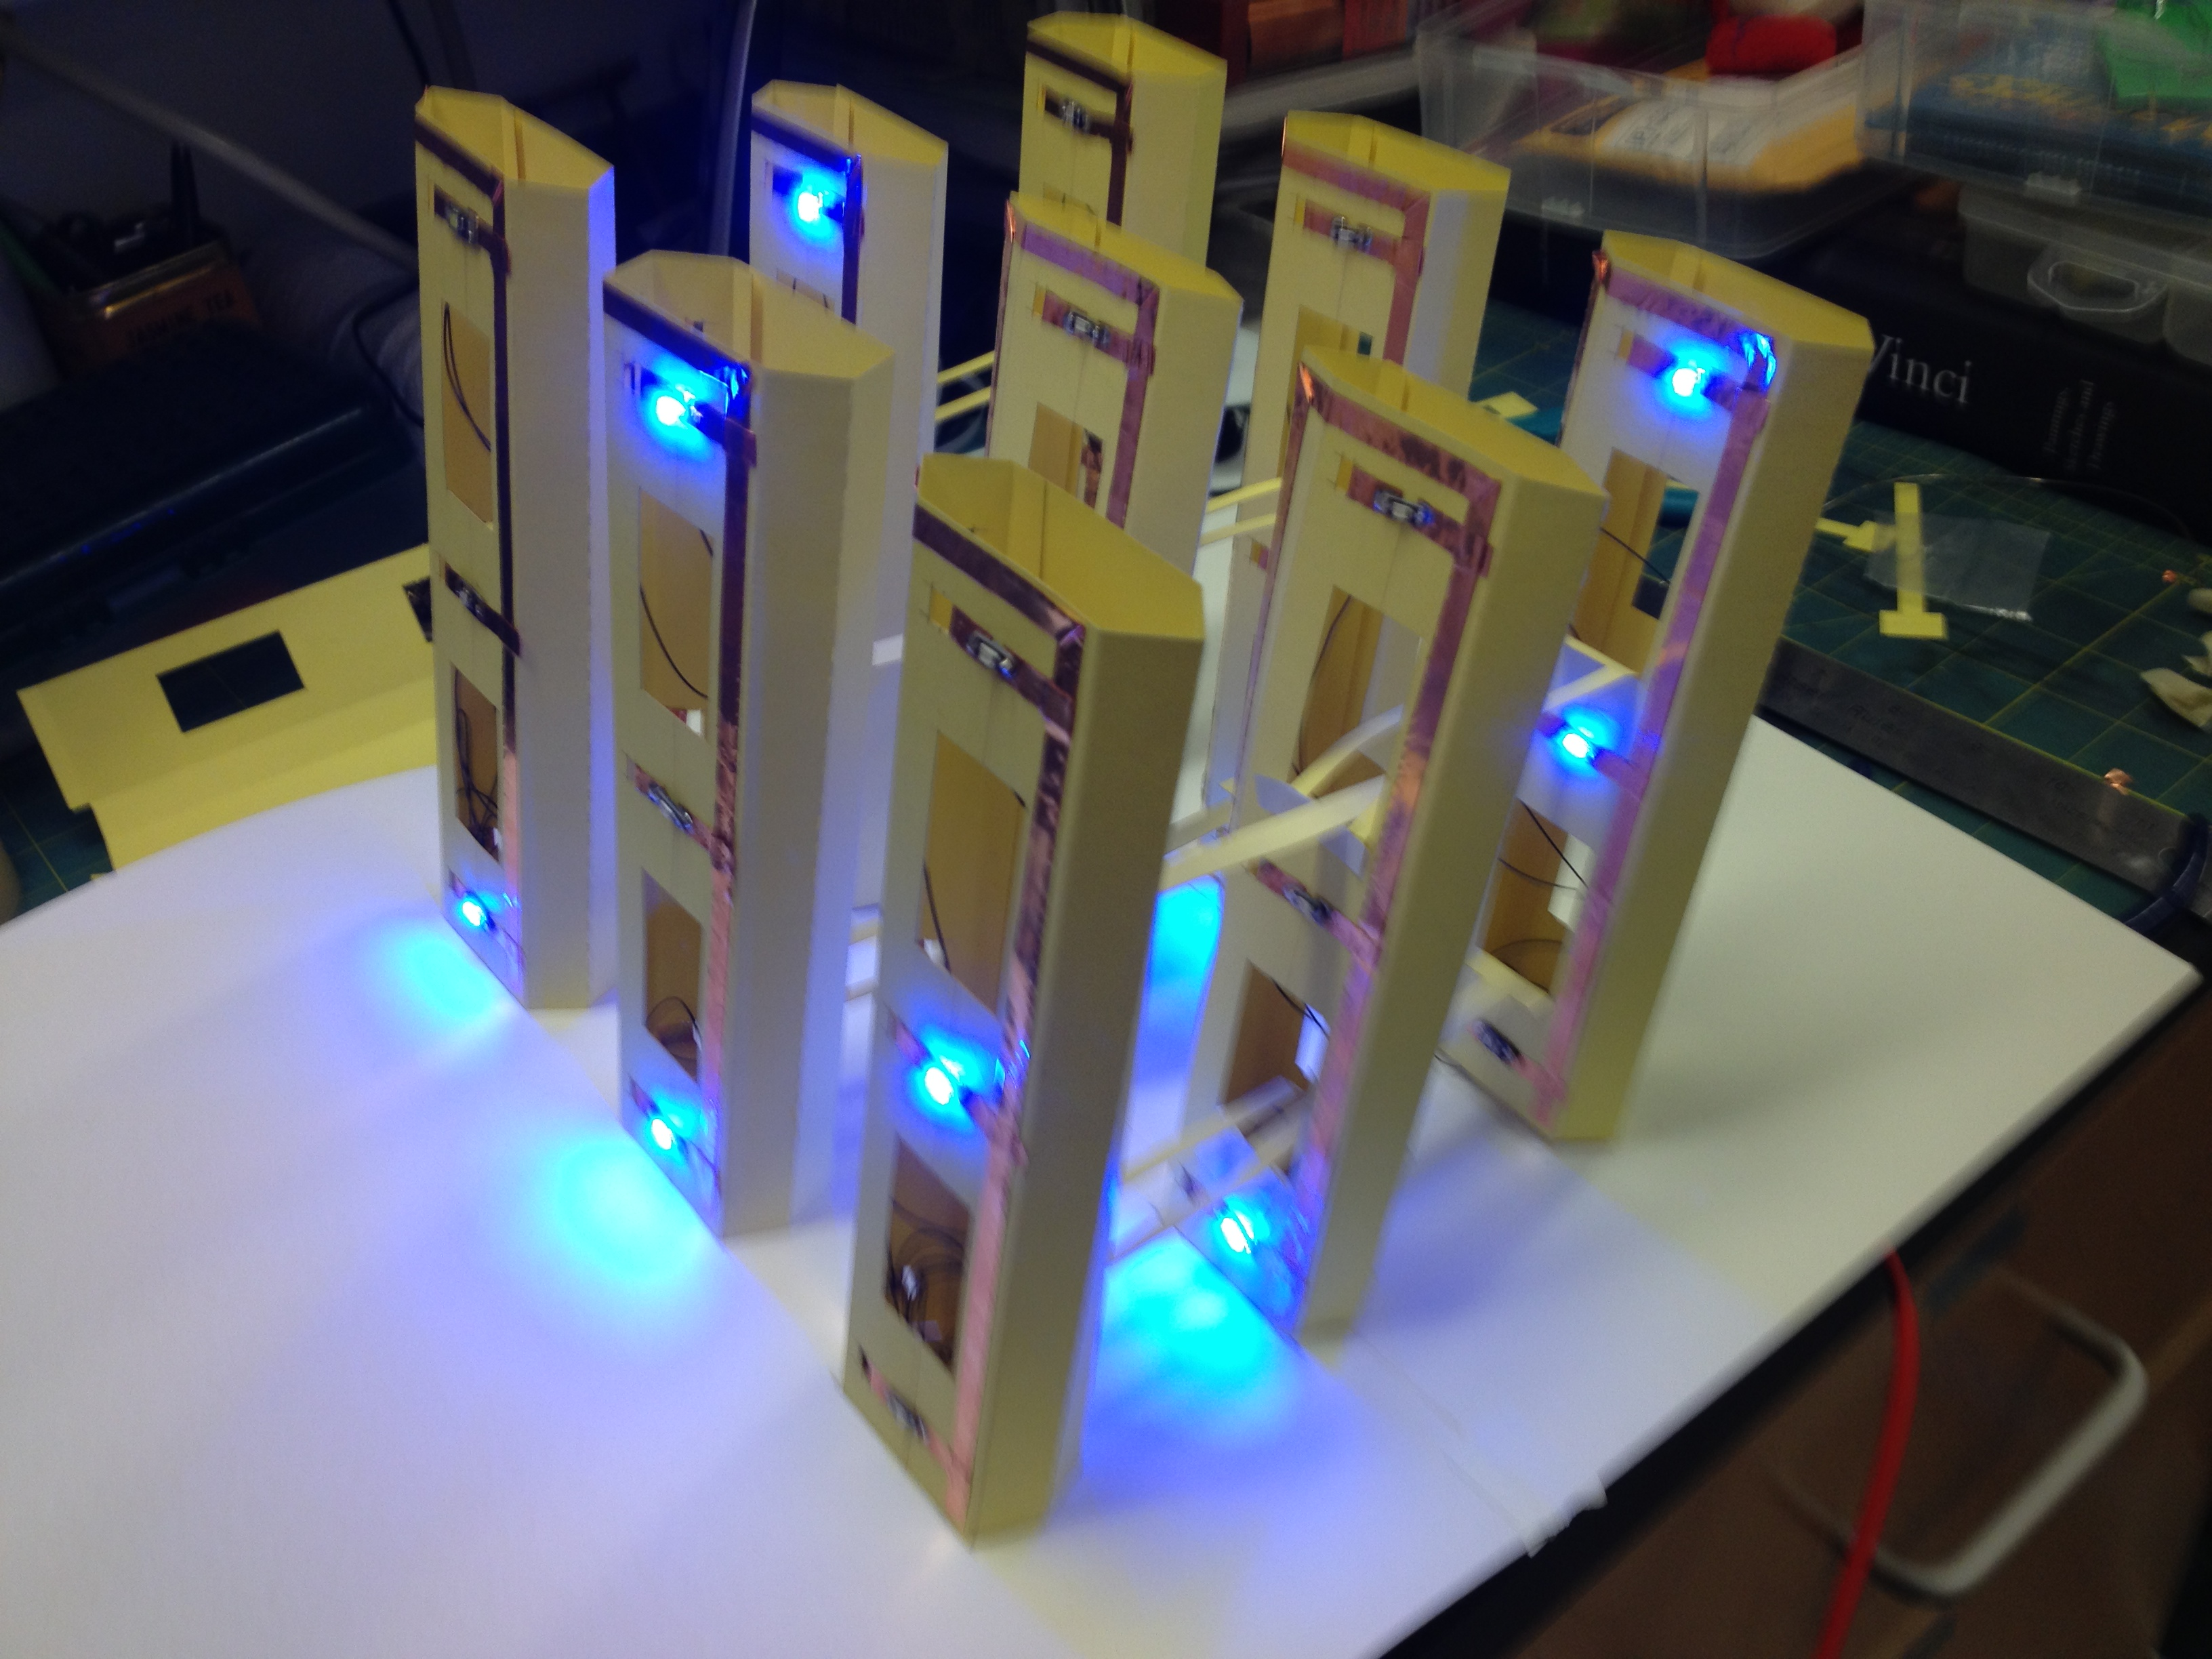
\includegraphics[width=.45\linewidth]{images/popup1} &
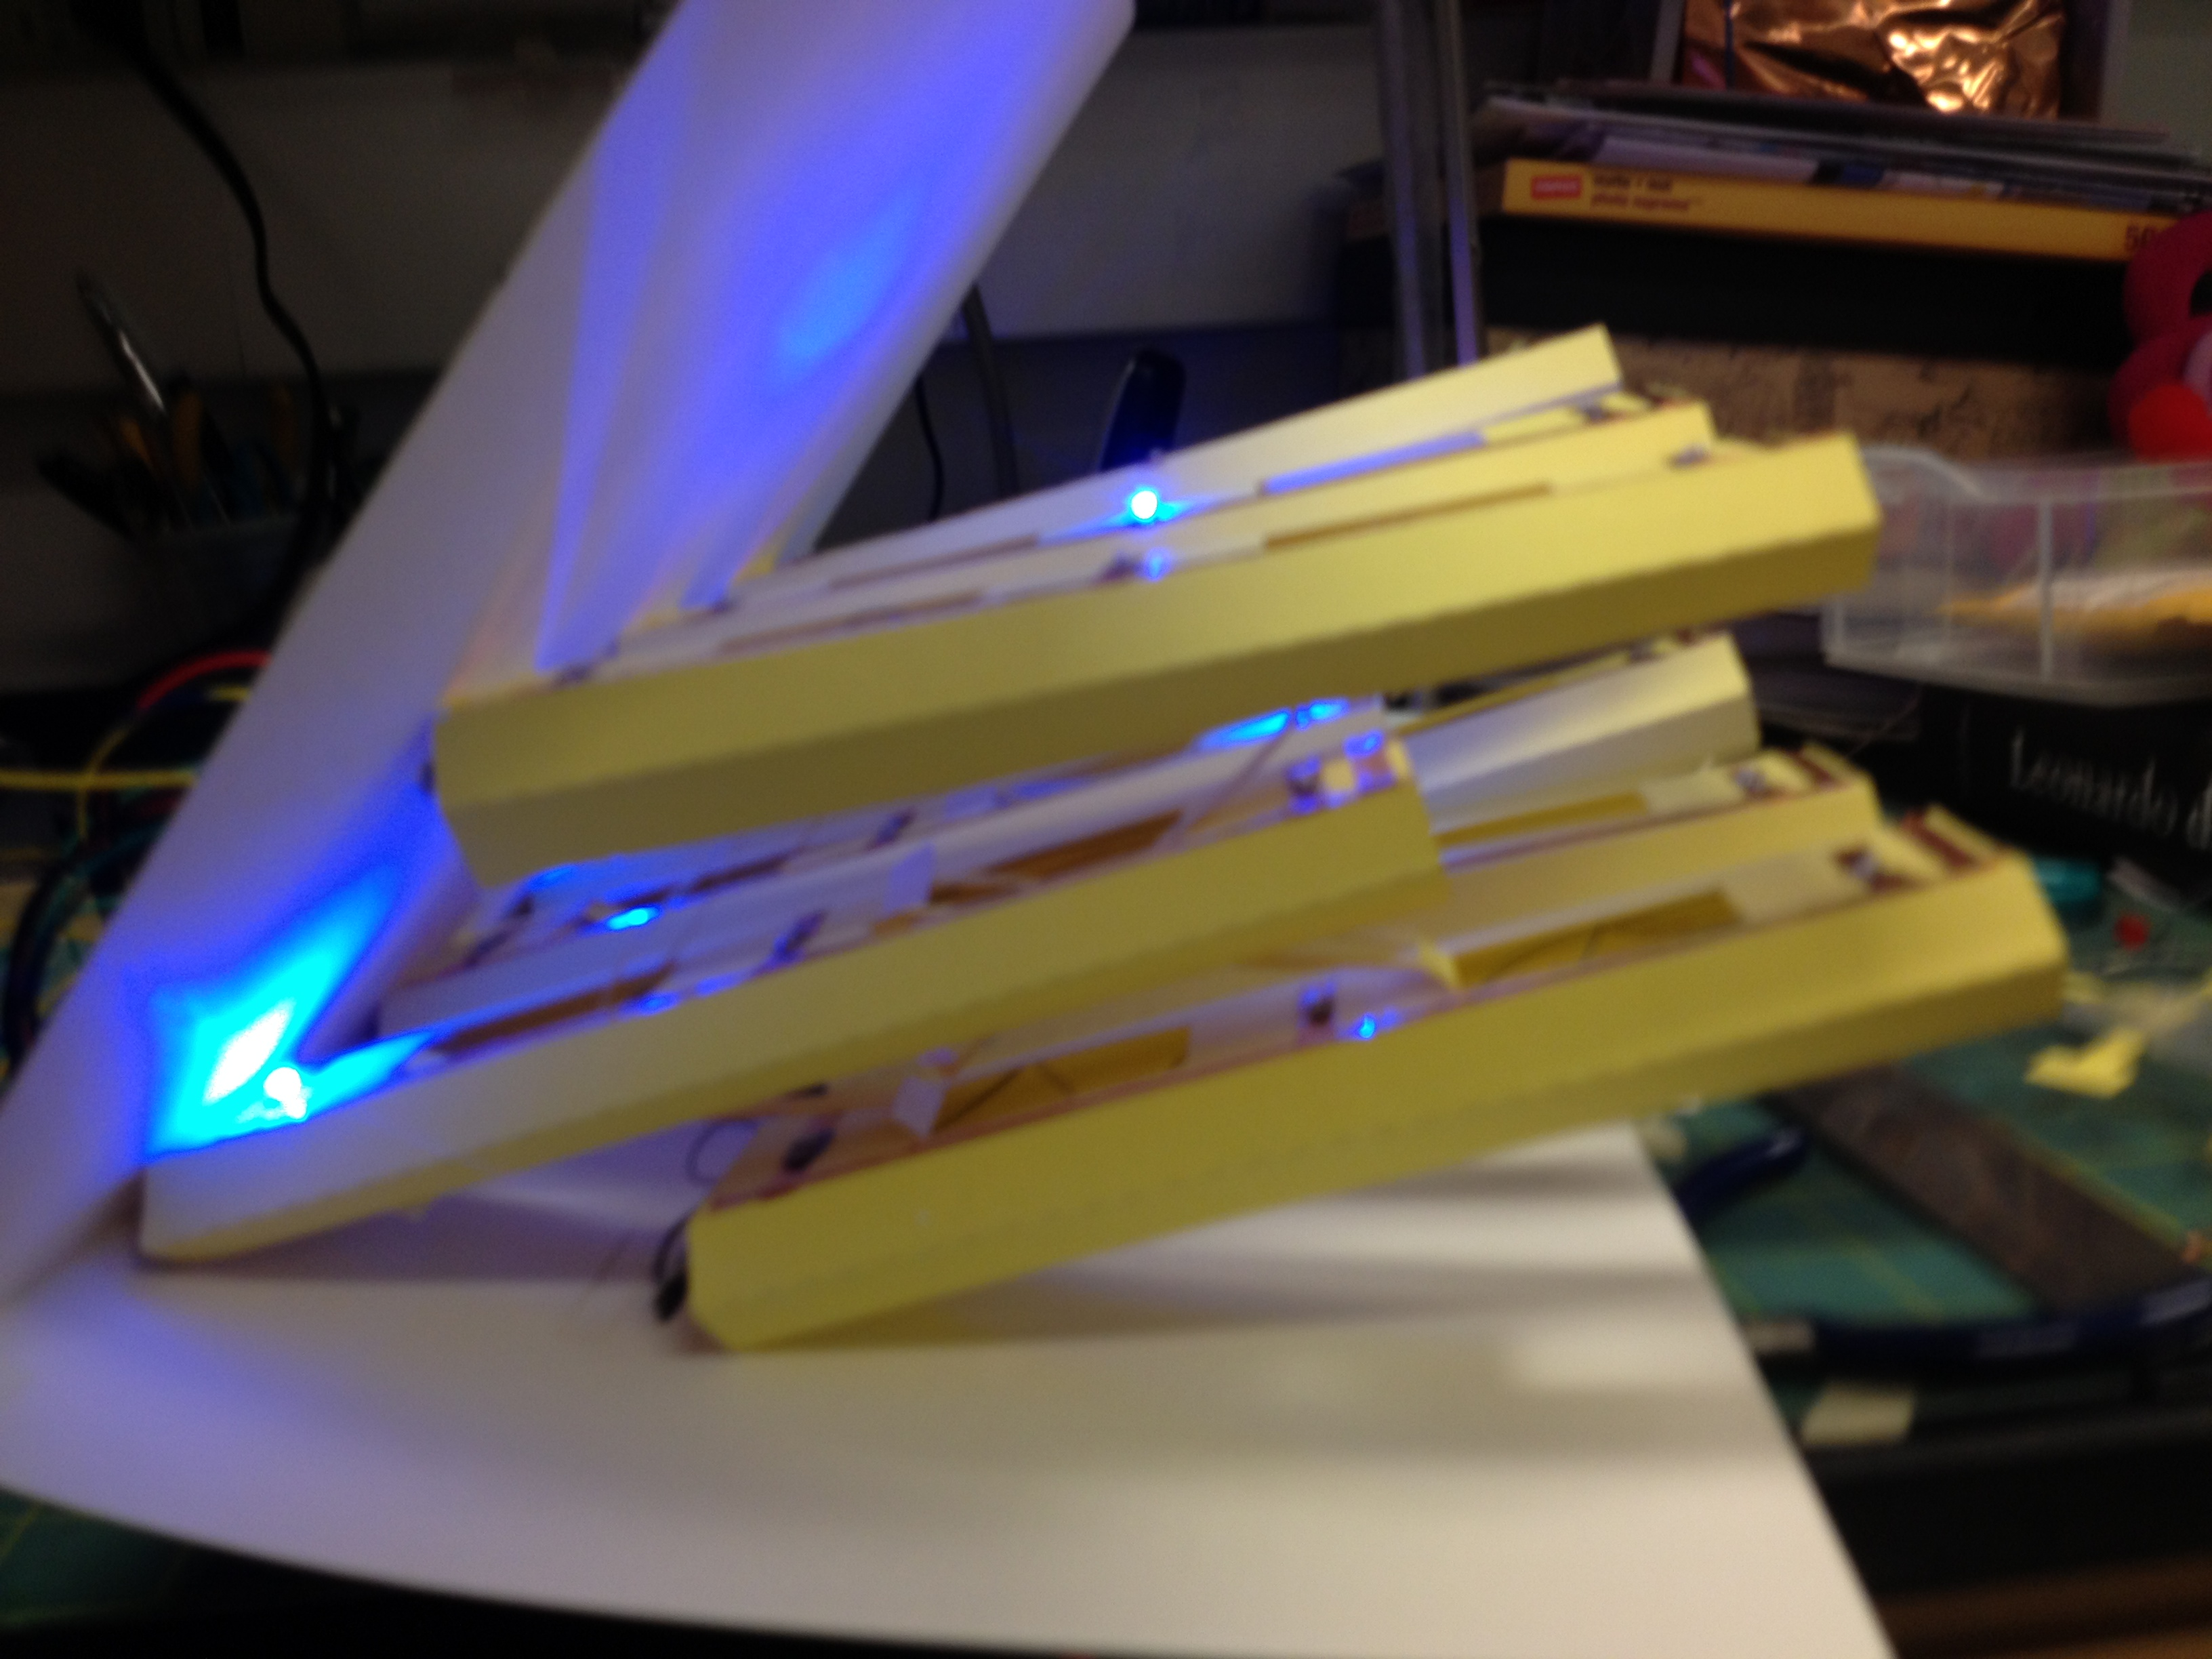
\includegraphics[width=.45\linewidth]{images/popup2}
\end{array}$
\end{center}
\caption{Two views of the pop-up book prototype, showing the paper towers and 
LEDs in both open and closed states.}
\label{fig:popup}
\end{figure}

Each tower has a copper tape circuit consisting of three LEDs on the front face
and three corresponding capacitive touch sensors on the left face. The copper
tape acts as a paper-friendly conductive material to connect the electronic
components together much like traditional wire. The LEDs are soldered onto the
copper tape for greater stability. The capacitive sensors are simply a piece of
copper tape which is connected to a pin on a microcontroller (in the first
version, this is an Arduino Mega Pro). By bringing the internal pull-up resistor
connected to the pin `LOW' (to ground) and then timing how long it takes to get
back to a `HIGH' state we can tell if the connection is being influenced by a
capacitive force. For example, if there is no interference on the circuit, the
timer will normally only get to `1' before the resistor is back to a HIGH state;
if a finger is placed on the copper tape, the reading will be
much higher (typically around `17'). Based on this change, we can detect which
switch was touched and toggle the associated LED on or off. The hollow interior
of each paper tower is used to solder thin 30-gauge wire to the three LEDs, the
three switches, and ground. These seven wires are soldered to a row of headers
that stick through the bottom of the first layer of the pop-up book. Wires are
then run along the backside of the top layer of paper from these headers to the
microcontroller. The entire circuit in then encased in a cloth-covered cardboard
binder that acts as a book cover as well as a means to protect and hide the
electronics.

The software originally written for the UCube and SnapCAD was adapted to work
with the pop-up book, making it capable of similar types of algorithmic modeling
and stereolithography output for 3D printing. As the grid is 3x3x3, it also
makes sense to adapt some of the game-playing aspects of the larger devices
(e.g., it would still be possible to play 3D tic-tac-toe). In addition to adding
this functionality, there are several improvements and finishing touches to be
made on the book itself. Additionally, the current hardware setup for the pop-up
book does not allow for the LED's to be snapped on or off, making certain
multi-player or multi-shape operations impossible. Weather or not this
functionality is crucial to the pop-up book will determine if changes need to be
made.  

Given the different medium of the pop-up book (paper as opposed to circuit
boards), it is worth exploring the possibilities afforded by a cheaper, more
flexible material. For instance, the flexibility of paper might provide the
means for new types of modeling actions. It is plausible to imagine paper tabs
or other mechanisms that perturb the LEDs off the integer lattice, or alter the
overall topology in such a way that new shapes are possible (e.g. by deforming
an equidistant grid into a spherical shape). There may be additional sensors or
hardware that could be embedded into the book to provide new functionality
(rotation, proximity, pressure). Additionally, due the inexpensive and portable
nature of the pop-up book, it is worth exploring the sorts of interactions that
could occur between several pop-up books (e.g., extending the input field to
include two or more grids, networked interactions like cooperative modeling
tasks, or competitive games like 3D-battleship). By using paper as a material to
think with, we may find further possibilities as development continues.

\section{Software}
Put stuff about software development here. Details. Screenshots.